% ICDE 2027 R2 - IEEE 双栏格式（anti-defensive-writing 优化版 + 去工程化修订：叙事重构，数据/图表不变）
% 编译: pdflatex main_icde_press.tex; 严格匿名版
\documentclass[conference]{IEEEtran}
\usepackage{graphicx,amsmath,amssymb,booktabs,multirow,amsthm,cite}
\usepackage{tikz}
\usetikzlibrary{arrows.meta,calc}
\definecolor{cNavy}{HTML}{2F3B52}
\definecolor{cGreenD}{HTML}{3F6B52}
\definecolor{cGreen}{HTML}{7FB69B}
\definecolor{cGreenL}{HTML}{ECF7F1}
\definecolor{cPurpD}{HTML}{5C4B7D}
\definecolor{cPurp}{HTML}{9B8FC0}
\definecolor{cPurpL}{HTML}{EDE6F6}
\definecolor{cBlueL}{HTML}{EAF1F8}
\definecolor{cRedL}{HTML}{FDECEC}
\definecolor{cAccR}{HTML}{D9534F}
\definecolor{cAccG}{HTML}{43A047}
\definecolor{cAmber}{HTML}{F0A93B}
\definecolor{cGrayT}{HTML}{6B7280}
\definecolor{cBlue}{HTML}{4A7EB5}
\definecolor{cViolet}{HTML}{8B6FB8}
\definecolor{cOrange}{HTML}{E08A3C}
\DeclareMathOperator{\Var}{Var}
% \paragraph is used only as an unnumbered run-in heading; stop IEEEtran's
% "a) b) c) ..." paragraph lettering (levels below subsection print no number)
\setcounter{secnumdepth}{3}
\newtheorem{theorem}{Theorem}
\newtheorem{lemma}{Lemma}
\newtheorem{proposition}{Proposition}
\newtheorem{remark}{Remark}
\title{What Can a Single Table Tell About Its Missingness Mechanism?\\
Testable Limits, a Diagnostic, and a Benchmark}

\author{
\IEEEauthorblockN{Nan Hu, Xueqiong Li, Huibin Tan, Guijian Tang, Huang ziyin, Ji Wang}
\IEEEauthorblockA{\textit{School of Computer Science} \\
\textit{National University of Defense Technology} \\
Changsha, Hunan}
}
\begin{document}
\maketitle

\begin{abstract}
Before choosing how to handle missing values, a practitioner is told to ask \emph{why} they are
missing. No tool answers that question with a calibrated, per-table probability. This paper
settles what a \emph{single} incomplete table can and cannot reveal about its missingness
mechanism, and builds the tools that respect that boundary.
(i)~\emph{Theory.} For two-pattern laws the observed law places exactly one non-trivial
restriction on the mechanism: pattern homogeneity (MCAR-rationalizability). Above it everything
detaches: one observed law admits MAR and genuinely-MNAR generators, and no pooled
residual-shape test can separate them. For self-selection on a predictable column the pooled
residuals are exactly extended skew-normal, with an attenuation law validated to a median
skewness deviation of $0.008$. Selection strength is link-relative, with a link-invariant
quantile contrast in closed form.
(ii)~\emph{Benchmark.} MechZoo: six base and three held-out mechanism families, real-table
injection, and a joint-shift cell that turns the boundary into a reproducible measurement.
(iii)~\emph{Diagnosis.} MissDx, a zero-shot diagnostic over the testable hierarchy, beats a
pattern-targeted moment test on MCAR detection by $+4.6$--$5.5$\,pp AUROC, is calibrated
in-distribution (fine-grained ECE $0.03$--$0.04$), and concentrates its entropy on the
unidentifiable boundary class. Outside the training families, on the MAR-vs-MNAR level, no
evaluated system stays above the majority-class baseline, and the diagnostic's calibration error
tracks the shift (coarse ECE $0.22$ on real tables, $0.31$ under joint shift). This declared
validity domain, not silent extrapolation, is what makes the diagnostic actionable.
\begin{IEEEkeywords}Missing data mechanisms, MCAR/MAR/MNAR, identifiability, mechanism diagnosis, benchmark\end{IEEEkeywords}
\end{abstract}



\section{Introduction}
Missing data is the default condition of tabular data. Four decades of taxonomy (MCAR, MAR, MNAR
\cite{rubin1976}) and a recent wave of deep imputers share one premise: the \emph{mechanism} of
missingness is known or irrelevant, and the task is to fill values. Yet the choice of
treatment (impute, model the missingness explicitly, or leave entries absent) depends exactly on
the mechanism: the same action is unbiased under MCAR, requires conditioning under MAR, and is
systematically biased under MNAR, and no tool delivers a calibrated, per-table answer.

\paragraph{Example.} Consider a clinical table where the lab-result column has $25\%$
missingness. If the values are MCAR (lab machine failures), simple mean imputation is
unbiased. If MAR (sicker patients get more tests, so the \emph{observed} severity score
predicts missingness), the analyst should condition on that score. If MNAR (the lab test
itself is ordered only when the physician suspects an abnormal result, so high values are
selectively missing), \emph{no single-table method} can distinguish this from MAR without
distributional assumptions. Imputing from observed values then systematically underestimates
the true burden. The diagnostic we build tells the practitioner which of these
regimes she is in, with a calibrated posterior and a declared validity domain; our theory
tells her where no such tool can exist.

The state of the art offers three unsatisfactory answers. Little's $\chi^2$ test \cite{little1988}
probes one global hypothesis with asymptotic calibration. Pattern-specialized
imputers \cite{feitelberg2025} train per-pattern specialists but \emph{assume the pattern is
known}; their own introduction concedes that distinguishing MAR from MNAR ``using the observed
data alone is generally impossible.'' Joint mask-value models \cite{diffjoint2026,missbgm2026}
fit per dataset, fail in the small-sample regime where diagnosis matters, and output
entry-wise labels rather than mechanism posteriors. The methodological
fallback is a sensitivity analysis over departures from MAR \cite{mk2007}; what is missing is
the object such an analysis needs first: a statement of how far the observed table itself can go.

This paper asks the question underneath all of them: \textbf{what can a single incomplete table
tell about its missingness mechanism at all?} We answer with three interlocking contributions.

\textbf{A testable-hierarchy theory (Sect.~\ref{sec:theory}).} For two-pattern laws the observed
law carries exactly one non-trivial restriction: pattern homogeneity, i.e.\ MCAR-rationalizability;
everything above it detaches, and we construct both an MAR and a genuinely-MNAR generator for the
same observed law (Lemma~\ref{lem:dual}). For self-selection on a conditionally predictable column
we give an exact extended-skew-normal (ESN) characterization of the pooled observed residuals with
an explicit attenuation law (Lemma~\ref{lem:esn}), validated on oracle residuals at a median
deviation of $0.008$ skewness (Sect.~\ref{sec:exp-validate}); and an impossibility result: a test
whose population limit is a functional of the pooled re-fit residuals cannot be consistent against
MAR/MNAR (Lemma~\ref{lem:pooled}). The latter explains why residual-skewness truncation
diagnostics are fragile; it does not cover moment tests or conditional-shape tests.
Selection-strength is link-relative (Prop.~\ref{prop:link}); the classical probit/logit $1.7$
rescaling is recovered in a closed-form link calculation.

\textbf{MechZoo (Sect.~\ref{sec:bench}).} Six base families, three held-out families differing in
functional form, driver structure, and shape, with labels derived from the mechanism actually
applied; real tables with injected mechanisms; and a \emph{joint-shift cell} (real tables
$\times$ held-out families) that, to our knowledge, no prior benchmark isolates.

\textbf{An amortized diagnostic (Sect.~\ref{sec:missdx}).} Per-column diagnostic statistics
(observed data only) aggregated by a set-attention encoder into a posterior over the hierarchy.
Its claimed properties are stated before the experiments and verified there: it beats a
pattern-targeted moment test on MCAR detection, its posterior is calibrated in-distribution,
and its entropy localizes on the unidentifiable boundary class. Its declared validity domain
is part of the output.

Our evaluation closes the loop between theory and measurement. On real tables and under joint
shift, on the MAR-vs-MNAR level, no system we evaluate---MissDx, either linear probe, Heckit,
or a tabular foundation model---is reliably above the majority-class baseline, precisely the
collapse that Proposition~\ref{prop:hier} predicts for the unidentifiable levels; on the
testable MCAR-detection level the linear probes clear the same baseline by $7.0$\,pp on real
tables. A
mechanism-to-treatment routing experiment shows that the bottleneck at realistic sample sizes
is the insensitivity of standard imputation policies, not the diagnosis, which is why the
routing rule we derive falls back to bounding and sensitivity analysis. The theory explains
each measurement, and Sect.~\ref{sec:disc} makes the resulting open problem precise.

\paragraph{Contributions.} (1)~\emph{Theory}: a testable hierarchy for single-table
missingness-mechanism diagnosis, with constructive dual rationalization (Lemma~\ref{lem:dual}),
an exact ESN characterization with a predictively validated attenuation law
(Lemma~\ref{lem:esn}), and a pooling impossibility result (Lemma~\ref{lem:pooled}).
(2)~\emph{Benchmark}: MechZoo, a mechanism-labelled benchmark with 9 families, 5 evaluation
cells spanning synthetic and real tables, and a joint-shift cell that stress-tests
distribution robustness. (3)~\emph{Diagnostic}: MissDx, a zero-shot diagnostic over the
testable hierarchy that outperforms the classical moment test on MCAR detection
($+4.6$--$5.5$\,pp AUROC), with per-column feature attribution, entropy localization on the
boundary class, and a declared calibration domain. (4)~\emph{Actionability}: a per-column routing rule (impute, bound, or sensitivity
analysis) derived from the hierarchy, whose validity conditions are the theorem statements
themselves. (5)~\emph{Boundary results}: preregistered
measurements that locate, under controlled shift, where single-table diagnosis ends---mechanism
labels and calibration do not transfer beyond the generator families they were learned on, and
treatment routing at realistic sample sizes is bounded by the insensitivity of the imputation
policies, not by the diagnosis. MechZoo makes both measurements reproducible.


\section{Related Work}
\paragraph{Data management.} Data-quality systems routinely profile completeness as a
first-class metric; HoloClean \cite{holoclean2017} and subsequent repair pipelines consume
missingness signals without modelling their generating mechanism. Our result sharpens this
interface: the only trustworthy signal a profiler can emit from a single table is the
homogeneity layer (plus its per-column attribution); above that, the right output is a
calibrated posterior with a declared validity domain. MissMecha \cite{missmecha2025} provides
mechanism simulation and MCAR testing for mixed-type tables; our benchmark complements it
with mechanism-family labels, held-out families, and the joint-shift cell.

\paragraph{Statistics.}
Little's test and MCAR diagnostics \cite{little1988}; selection models and their score tests
\cite{heckman1979,dk1994}; identifiability of missingness models
\cite{rubin1976,seaman2013,mk2007,ceriscioli2026}, and the complementary question of which
queries remain recoverable under a missingness graph \cite{mohanpearl2021}. Because MAR is
untestable, the methodological literature answers the practitioner with a sensitivity analysis
over departures from MAR (delta-adjusted multiple imputation, pattern-mixture and tipping-point
analyses) \cite{mk2007,noonan2022}, not with a mechanism label. Testing MAR
from data has its own line \cite{tian2015}, which buys testability with graphical structure
across variables; our impossibility results (Lemmas~\ref{lem:dual}--\ref{lem:pooled}) price
what single-table statistics can reach. Our results fit this
division of labour rather than displacing it: a single table cannot deliver the label, so we
deliver a calibrated posterior together with an explicit statement of its validity domain.

For systems, data-cleaning and data-quality pipelines \cite{holoclean2017} are the natural
consumers of a mechanism diagnostic; pattern-specialized and joint imputers
\cite{feitelberg2025,diffjoint2026,missbgm2026,tabsoda2026} assume the pattern or fit a mask-value
model per dataset; incomplete-data causal discovery \cite{missnodag2026,misscnf2026,pairci2026}
uses missingness structurally; and \cite{feitelberg2025} carries a missing-data benchmark. The
equivalence insight we build on is Rubin's and classical. Our additions are narrower: a
self-contained two-pattern construction, the pooled-residual ESN characterization with an explicit
attenuation law, and a benchmark cell (real tables $\times$ held-out families) that, to our
knowledge, no prior benchmark isolates.


\section{What Is Testable: The Hierarchy}\label{sec:theory}

\begin{figure*}[t]
\centering
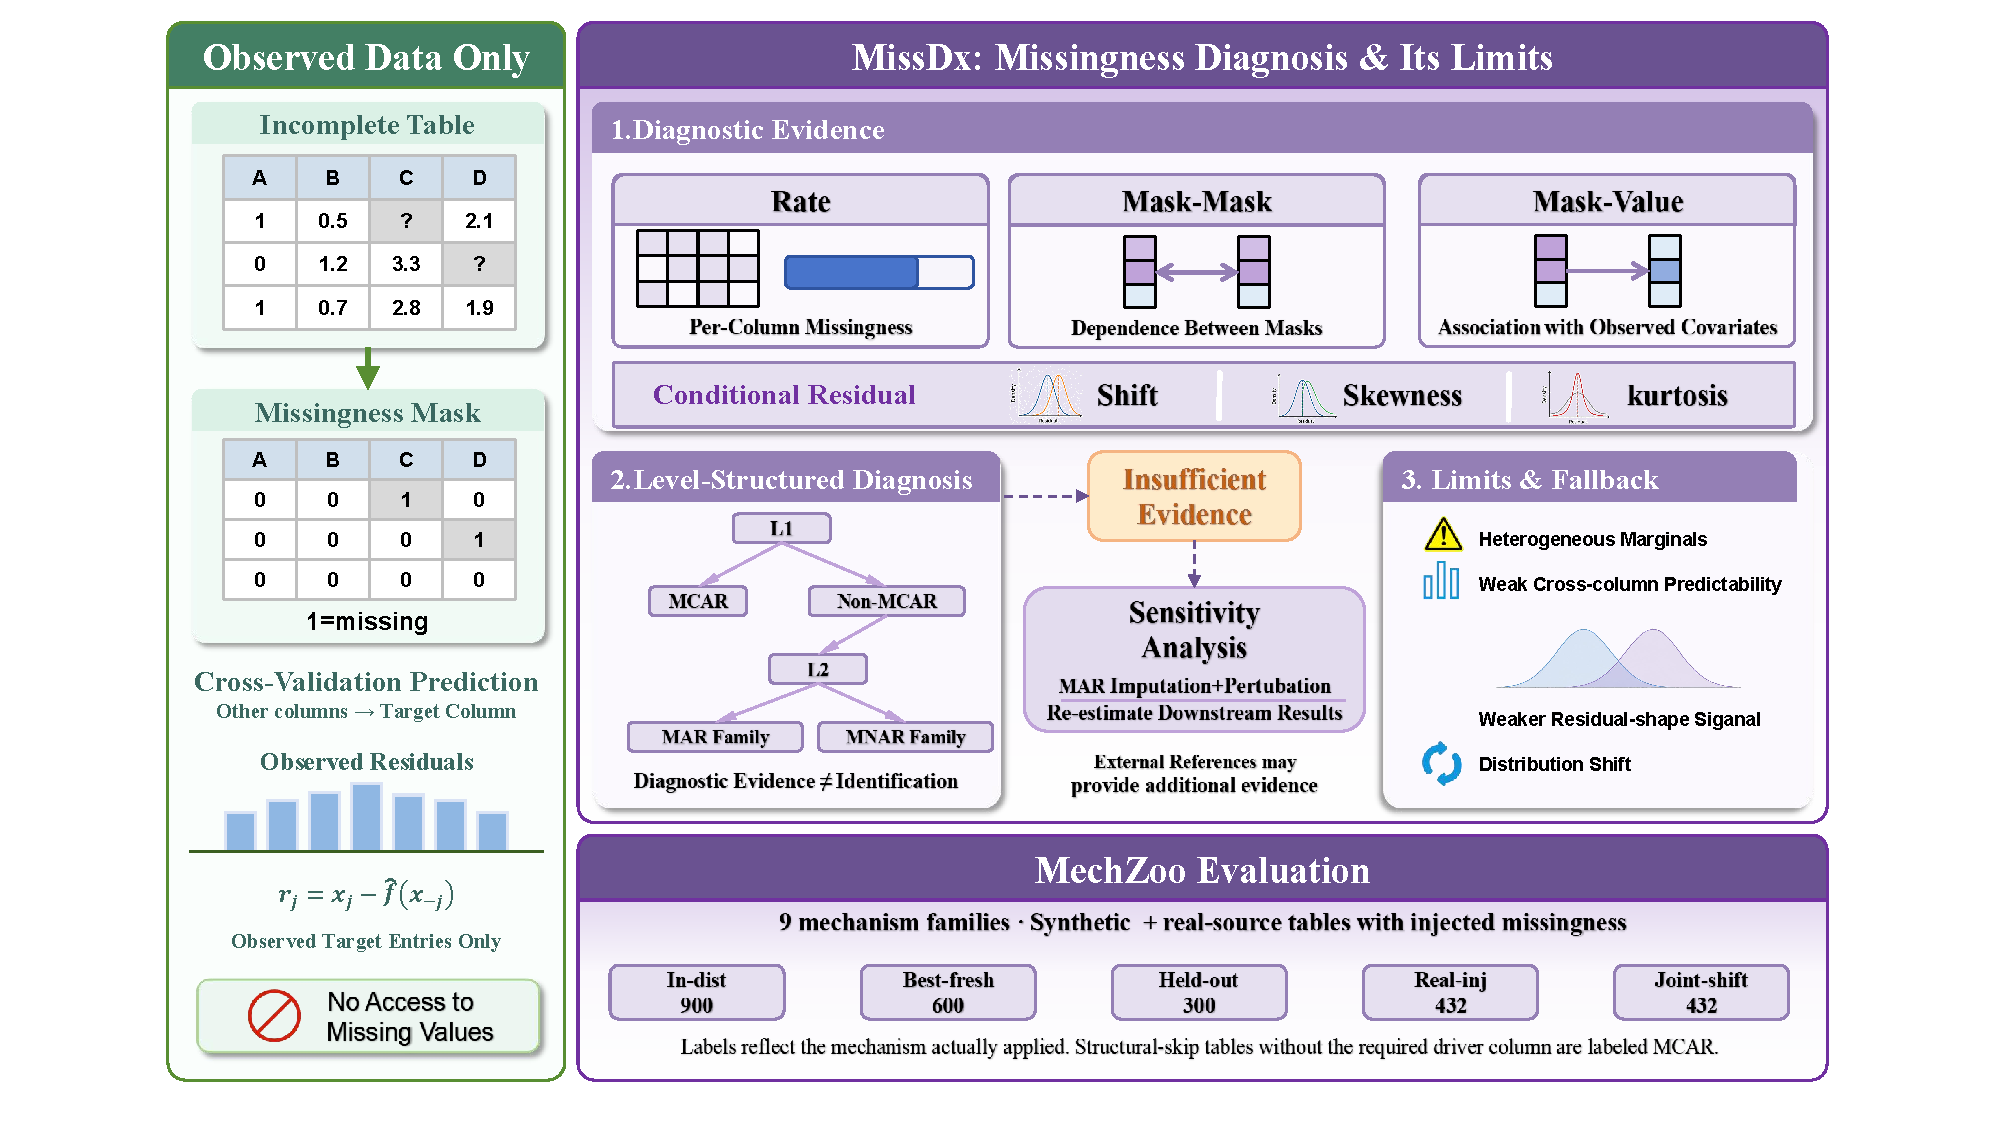
\includegraphics[width=\textwidth]{figs/2.pdf}
\caption{\textbf{Overview of MissDx and the limits of missingness diagnosis from observed data.} An incomplete table and its missingness mask provide three diagnostic channels: missingness rate, mask--mask dependence, and mask--value dependence. Cross-validated predictions from other columns additionally yield observed residual summaries that probe conditional distributional shape. These features support level-structured diagnosis, first separating MCAR from non-MCAR mechanisms and then distinguishing MAR-family from MNAR-family mechanisms. Such predictions are not identification guarantees: heterogeneous marginals can undermine parametric assumptions and within-table references, while weak cross-column predictability attenuates residual-shape signals. MechZoo evaluates diagnosis across synthetic and real-source tables with injected mechanisms, including held-out families and joint shifts. Where the evidence is insufficient, sensitivity analysis provides a fallback rather than a definitive mechanism assignment.}\label{fig:hierarchy}
\end{figure*}
Fig.~\ref{fig:hierarchy} gives an overview of the diagnostic pipeline and where its evidence ends. This section
makes each level precise, working upward from the always-observable rates through the testable
homogeneity layer to the unidentifiable MAR/MNAR boundary.
\paragraph{Setting.}
$X=(X_1,\dots,X_d)\sim P_X$ with masks $M$ generated by $P(M\mid X)$; the analyst observes
$(X_{\mathrm{obs}},M)$; the \emph{observed law} is their joint distribution. Two generators are
\emph{observationally equivalent} if they induce the same observed law; any test's power flows
only through the observed law.

\begin{proposition}[Hierarchy]\label{prop:hier}
(i) MCAR $\Rightarrow$ pattern homogeneity: there is a common $Q$ such that each pattern's
observed conditional law equals the corresponding marginal of $Q$; Little's test probes the moment
content of homogeneity, a necessary implication. The converse fails (self-selection on a
coordinate missing within a pattern is absorbed by $Q$). (ii) For two-pattern laws, the only non-trivial restriction the observed law places on
mechanisms is homogeneity; its negation is detectable and locally
attributable (which columns $\times$ patterns drift). Genuine MAR-dependence itself is never
testable: every two-pattern observed law has an MAR rationalization, and when
$\mathrm{supp}\,\tilde\mu^0\subseteq\mathrm{supp}\,\tilde\mu^1_{x_1}$ it also has a genuinely-MNAR
twin (Lemma~\ref{lem:dual}). The multi-pattern statement is classical
\cite{rubin1976,mk2007} and is cited rather than reproved; every result in this paper is a
two-pattern result. (iii) Consequently the MAR/MNAR distinction detaches from the observed law (Lemma~\ref{lem:dual}).
\end{proposition}

\begin{lemma}[Dual rationalization; monotone dropout]\label{lem:dual}
Let patterns $m^0$ (observe $x_1$) and $m^1$ (observe $x_1,x_2$) have observed sub-distributions
$\tilde\mu^0,\tilde\mu^1$ with $\{x_1:\tilde\mu^0>0\}\subseteq\{x_1:\tilde\mu^1_{x_1}>0\}$.
Only the shared coordinates are used, so the construction extends to any two-pattern law with
overlapping support; the monotone case is written for concreteness.
\emph{(MAR side)} With
\begin{equation}
\lambda_S=\tilde\mu^0_S+\tilde\mu^1_S,\qquad
h_k=\frac{d\tilde\mu^k_S}{d\lambda_S},\qquad
s_k(x)=h_k(x_S),
\label{eq:mar_constr}
\end{equation}
the conditional-coupling completion rationalizes the law and is MAR.
\emph{(MNAR side)} For any bounded Markov kernel $\rho(x_2|x_1)$ that is non-singular
($m(x_1)=\int\rho\,d\tilde\mu^1>0$ where $\tilde\mu^0>0$) and non-degenerate, define
\begin{equation}
\varphi=\frac{\tilde\mu^0\,\rho}{m},\qquad
g=\frac{\varphi}{1+\varphi},\qquad
p'=\tilde\mu^1(1+\varphi).
\label{eq:mnar_constr}
\end{equation}
The selection $g$ depends on $x_2$ (the coordinate missing under $m^0$), so this is a
genuinely-MNAR rationalization. Hence no level-$\alpha$ test of any MAR-containing null has power above $\alpha$
at such MNAR points.
\end{lemma}

\begin{lemma}[ESN characterization and attenuation]\label{lem:esn}
Let $X_j=f(X_{-j})+\varepsilon$, $\varepsilon\sim N(0,\sigma^2)\perp X_{-j}$,
with $f(X_{-j})$ Gaussian and $\tau_f^2=\Var f(X_{-j})$, and
\begin{equation}
P(\mathit{miss}\mid X_j)=\Phi(a+bX_j),\qquad b\ne0.
\label{eq:selection_model}
\end{equation}
The pooled observed-residual density is
\begin{equation}
f_{\mathrm{obs}}(r)=\frac{\varphi_\sigma(r)\,\Phi(\alpha_0+\alpha_1 r)}
{\Phi\!\left(\alpha_0\middle/\sqrt{1+\alpha_1^2\sigma^2}\right)},
\label{eq:esn_density}
\end{equation}
i.e., an extended skew-normal $\mathrm{ESN}(0,\sigma,\alpha_1\sigma,\alpha_0)$ with
\begin{equation}
\alpha_1=\frac{b}{\sqrt{1+b^2\tau_f^2}},\qquad
\alpha_0=\frac{a+b\mu_f}{\sqrt{1+b^2\tau_f^2}},
\label{eq:attenuation}
\end{equation}
(up to the observe-side sign). For non-Gaussian $f(X_{-j})$ the weight is a convolution
smoothing without closed form; the identity is the Gaussian case. At $\alpha_0=0$ the skewness sign is $\mathrm{sign}(b)$ with the
classical skew-normal magnitude. The law $\alpha_1\to0$ as $\tau_f^2\to\infty$ is the
\emph{attenuation law}: the more of the column's variance sits in its predictable component, the
weaker the observable imprint of self-selection. Figure~\ref{fig:esn} validates
Eq.~\eqref{eq:attenuation} empirically.
\end{lemma}

\begin{lemma}[Pooled shape tests cannot be consistent]\label{lem:pooled}
Fix a fitting procedure whose population limit on selected rows is the conditional mean (correctly specified least squares or a consistent nonparametric regressor), and let $q^\ast$ be the population pooled re-fit residual law of a self-selection generator (finite first moment). There exists a structured MAR generator
\begin{equation}
\varepsilon'\sim q^\ast,\quad \varepsilon'\perp X_{-j},\quad P(M{=}1\mid X)=s'(X_{-j}),
\label{eq:mar_generator}
\end{equation}
whose pooled re-fit residual law is exactly $q^\ast$ (centered). Hence any functional $T$ of the pooled re-fit residual law with $T(F)=T(F*\delta_c)$ for all translations $c$ (skewness, kurtosis, quantile shapes) takes equal values on the pair:
\begin{equation}
T\bigl(q^\ast_{\mathrm{MNAR}}\bigr)=T\bigl(q^\ast_{\mathrm{MAR}}\bigr).
\label{eq:pooled_match}
\end{equation} The restriction acts on one functional of the observed law: it does not cover mechanism tests that use the mask law (Little's test) or conditional shapes (Remark~\ref{rem:sep}).
\end{lemma}

\begin{remark}[Separable information is conditional]\label{rem:sep}
The selected conditional density is $\mathrm{ESN}(f(t),\sigma,b\sigma,a+bf(t))$; within the ESN
family a translation changes only the location parameter. Whenever $f$ takes two values on the
selected support, the MNAR conditional family is not a location family and cannot match any
structured-MAR law: the information exists, but only in \emph{conditional} shapes, not pooled
statistics.
\end{remark}

\begin{proposition}[Link-relative strength]\label{prop:link}
Throughout, $X_j$ has full support on $\mathbb{R}$ and the analysis is inside a parametric
selection model $P(\mathit{miss}\mid X_j)=\Phi(a+bX_j)$. The parameterization-free target is the
link-free selection curve $s(x)=P(\mathit{miss}\mid X_j=x)$;
$(g,a,b)\mapsto s$ is non-injective exactly on affine reparameterizations. Within the
probit--Gaussian model of Lemma~\ref{lem:esn} the latent scale is fixed by $\tau_f^2$, so $(a,b)$
is identified; $s$ itself is not point-identified from a single table under self-selection
(Lemma~\ref{lem:dual}), so the claim is link-relative. Probability links admit
no exact cross-link match: equality $g(a_1{+}b_1x)=\tilde g(\tilde a{+}\tilde b x)$ on all of
$\mathbb{R}$ forces $\tilde g=g\circ A$ for an affine $A$ (substitute $t=a_1{+}b_1x$), so exact
matches arise precisely within affine classes; probit/logit are $\varepsilon$-near (minimax scale $1.702$, maximum CDF
gap $0.0095$ \cite{haley1952,amemiya1981}), so strength is in-principle identified but practically
ill-conditioned across links; cross-link transfer must be phrased on link-invariant functionals
(e.g., the quantile contrast $s(q_{90})-s(q_{10})$).
\end{proposition}

\begin{remark}[Heckman's assumption, coordinatized]\label{rem:heckman}
The selection-model tradition \cite{heckman1979,dk1994} buys testability of self-selection with
distributional priors on $\varepsilon$. Lemmas~\ref{lem:esn}--\ref{lem:pooled} price it: without a
shape prior, the pooled imprint is exactly reproducible by an MAR generator; with Gaussian
$\varepsilon$ the imprint is ESN with an attenuation that can be arbitrarily weak.
\end{remark}


\section{MechZoo}\label{sec:bench}

\begin{table*}[t]
\caption{MechZoo mechanism families. Base families are used for training; held-out families
are never seen during training. Strength $b\sim U(0.7,3.0)$; rates are calibrated per table
to $[0.10,0.40]$ (intercept binary search) so rates cannot leak the label.}
\label{tab:mechzoo}
\centering\small
\begin{tabular}{llll}
\toprule
Family & Type & Selection function & Key parameters \\
\midrule
\multicolumn{4}{l}{\emph{Base (used for training)}} \\
MCAR & control & $P(m_j{=}1)=\pi$ & $\pi\in[.10,.40]$ \\
MAR-obs & MAR & $P(m_j{=}1)=\sigma(a{+}b\,z(x_k))$, $k\ne j$ & $b$; driver column $x_k$ \\
Self-mask & MNAR & $P(m_j{=}1)=\Phi(a{+}b\,z(x_j))$ & $b$ (sign $\pm$) \\
Latent-MNAR & MNAR & $P(m_j{=}1)=\Phi(a{+}b\,u)$, $u\perp X_{\mathrm{obs}}$ & $b$; loading $\lambda\in[.6,.95]$ \\
Structural skip & structural & $m_j=\mathbf{1}[x_k{=}v^*]$, categorical $k$ & driver value $v^*$ \\
Mixture & MNAR$+$MCAR & half rows MCAR($p$), half self-mask($b$) & $p\in[.05,.30]$; $b$ \\
\midrule
\multicolumn{4}{l}{\emph{Held-out (never trained on)}} \\
MAR-multi & MAR & $P(m_j{=}1)=\sigma(a{+}b_1z(x_{k_1}){+}b_2z(x_{k_2}))$ & $b_1,b_2$; two drivers \\
Logit self-mask & MNAR & $P(m_j{=}1)=\sigma(a{+}b\,z(x_j))$ & $b$; logit vs.\ probit link \\
Quantile censor & MNAR & $m_j=\mathbf{1}[x_j>q_\theta]$ w.p.\ $p_{\mathrm{hi}}$, else $p_0$ & $q\in[.5,.8]$; $p_0\in[.02,.08]$ \\
\bottomrule
\end{tabular}
\end{table*}

Table~\ref{tab:mechzoo} catalogues the nine mechanism families. Tables come from a generator
with deliberately heterogeneous marginals (Gaussian-mixture, $t_3$, log-normal), linear
cross-column dependence, and categorical columns; the heterogeneity carries the load: it is
what makes parametric priors misspecified and naive within-table references unreliable. A
structural-skip family whose driver column is absent degenerates to pure MCAR and is
relabelled as MCAR; this affects $4\%$ of synthetic tables and all nine real tables (for which we keep
numeric columns only, so no categorical driver exists). Nine public real tables receive injected
mechanisms: breast-cancer, diabetes, page-blocks, MagicTelescope,
balancing-scale, qsar-biodeg, wine-quality-white, synthetic-control, and ILPD. The nine
families span the three channels the theory isolates---rate, mask--mask, and
mask--value---with two families (MAR-multi, logit self-mask) that break the single-driver and
probit assumptions, and a censoring family whose semantics match laboratory detection limits.

\paragraph{Cells.} Table~\ref{tab:cells} lists the five evaluation cells. The real tables
contribute nine clusters of 48 near-replicates each; we treat them as correlated, not
independent. Table labels are computed from the mechanism actually applied, so a label always
names what generated the mask.

\begin{table}[t]
\caption{Evaluation cells. Every cell is generated by script from the seed shown, so all five
are reproducible without the real-table download; $k$ indexes the real source.}
\label{tab:cells}
\centering\small
\begin{tabular}{lrl}
\toprule
Cell & Tables & Construction \\
\midrule
in-dist & 900 & 6 base families, seed 999 \\
base-fresh & 600 & 6 base families, seed 777 \\
held-out & 300 & 3 held-out families, seed 778 \\
real-inj & 432 & 9 sources $\times$ 6 families, seed $500{+}k$ \\
joint-shift & 240 & 4 sources $\times$ 3 held-out, seed $900{+}k$ \\
\bottomrule
\end{tabular}
\end{table}

\section{MissDx: Amortized Diagnosis over the Hierarchy}\label{sec:missdx}

\begin{table}[t]
\caption{Per-column diagnostic features. All are computable from observed data only;
$f(x_{-j})$ is the cross-validated prediction of column $j$ from the other columns
($\hat\tau_f^2$ = fraction of column $j$'s variance explained by $x_{-j}$).}
\label{tab:features}
\centering\small
\begin{tabular}{llc}
\toprule
Feature & Formula & Cost \\
\midrule
Mask rate & $\bar m_j$ & $O(n)$ \\
Mask-mask $\phi$ & $\max_{k\ne j}|\mathrm{corr}(m_j,m_k)|$ & $O(nd)$ \\
Mask-value & $\max_{k\ne j}|\mathrm{corr}(m_j,x_k)|$ & $O(nd)$ \\
Residual shift & $|\overline{r_j}|$ where $r_j=x_j-\hat f$ & $O(nd^2)$ \\
Residual shape & $\mathrm{skew}(r_j)$, $\mathrm{kurt}(r_j)$ & $O(nd^2)$ \\
Skip $\chi^2$ & $\max_v V(m_j, \mathbf{1}[x_k{=}v])$ & $O(nd|\mathcal{V}|)$ \\
Type indicators & cont$/$bin$/$cat & $O(d)$ \\
\bottomrule
\end{tabular}
\end{table}

Per-column diagnostic statistics (Table~\ref{tab:features}; all computed from observed data
only): mask rate; mask-mask $\phi$; mask-vs-other-value correlations (the classical
heterogeneity channel); cross-prediction residual statistics; skip $\chi^2$. The dominant
cost is the cross-prediction step at $O(nd^2)$ for $n$ rows and $d$ columns ($d$ regressions,
each $O(nd)$); all other features are $O(nd)$ or cheaper, and the feature computation is
embarrassingly parallel across columns. A small set-attention aggregator without positional
encodings maps per-column
tokens to a posterior over the six base families plus a strength head; normalization constants
travel with the model. Trained once on MechZoo (24{,}000 synthetic tables), zero-shot thereafter. Trained on tables with $d\le12$ columns, it transfers to wider tables by tokenizing the first 12 columns: coarse-grain accuracy on synthetic wide tables is $.88$ ($d{=}20$), $.77$ ($d{=}50$), and $.80$ ($d{=}100$), against a $d{\le}12$ baseline of $.80$; it does not collapse on wide tables.
We make two claims for the diagnostic, stated here before the experiments and tested there:
(i)~\emph{in-distribution calibration}---fine-grained ECE $0.03$--$0.04$ for the learned
posterior, against $0.06$--$0.09$ for the value-probe; and
(ii)~\emph{entropy localization}---posterior entropy on the boundary class (latent MNAR)
exceeds that of decodable classes by $0.29$--$0.37$ nats (bootstrap 95\% CI $[+0.25,+0.34]$ on
the in-distribution pool). Sect.~\ref{sec:exp-levels} measures where these properties hold and
where they end, so the posterior's validity domain is a declared output of the system rather
than an implicit assumption.


\section{Experiments}\label{sec:exp}
\subsection{Level-Structured Results}\label{sec:exp-levels}

\paragraph{Protocol.} Cell sizes are 900 (in-distribution), 600 (base-fresh), 300 (held-out
families), 432 (nine real tables with injected mechanisms) and 240 (joint shift: four of the
nine real tables $\times$ three held-out families). L2 excludes MCAR-labelled tables, leaving
745/498/300/288/240. Labels are derived from the mechanism actually applied to each table, not
from the requested family: a structural-skip family whose driver column is absent degenerates to
pure MCAR and is labelled as such. This affects $4\%$ of synthetic tables and all nine real
tables, so 72 of the 432 real-injected tables are MCAR rather than MAR. All systems see the same pools and seeds; MissDx emits the argmax of its posterior; the
mask- and value-probes are multinomial logistic regressions trained on a disjoint pool (seed 21,
250 tables/class, 1{,}500 tables total); MissDx was trained once on 24{,}000 synthetic tables;
Heckit uses only continuous covariates, with one threshold calibrated on the training pool. Real
tables are never used in training; decision rules are fixed once and applied unchanged to all
cells. Table generators produce heterogeneous marginals (Gaussian-mixture, $t_3$,
log-normal), linear cross-column dependence, and categorical columns. The heterogeneity is
deliberate: it is what makes parametric priors misspecified and naive within-table references
unreliable. Mechanism strengths $b$ are drawn uniformly from $[0.7,3.0]$; missingness rates
are calibrated per table to a common band $[0.10,0.40]$ so that rates cannot leak the label.
The set-attention encoder has $h{=}128$, 2 layers, 4 heads ($0.25$M parameters); training is
12 epochs over 24{,}000 tables ($9{,}000$ steps, AdamW $10^{-3}$, cosine decay), taking
$\sim$190 seconds on one consumer GPU. All code, seeds, and result files are scripted;
we will release an anonymized artifact alongside the paper.
Three test-pool draws with a fixed model provide the seed variation. Training variance is
bounded by the $0.4$\,pp in-distribution macro-F1 gap between our two training runs.

Following the theory we report L1 (MCAR detection) and L2 (MAR-family vs MNAR-family among
non-MCAR) together with trivial baselines computed by script (Table~\ref{tab:levels}). Held-out
cells contain no MCAR family, so L1 is void there. In-distribution both levels clear the
trivial baselines (L1 $0.949$ vs $0.906$; L2 $0.858$ vs $0.753$). The deployment cells mark
the empirical boundary the theory predicts: on the L2 MAR-vs-MNAR decision no system we
evaluate---MissDx, either linear probe, Heckit, or a zero-shot tabular foundation model---is
reliably above the majority baseline on real tables or under joint shift
(Table~\ref{tab:levels} carries all values). On the testable L1 level, by contrast, the two
probes clear the baseline by $7.0$\,pp on real tables. Calibration tracks the same boundary
(Table~\ref{tab:calib_deg}): the
fine-grained ECE is $0.035$ in-distribution and undefined on the shifted cells, whose labels lie
outside the six-class vocabulary; at the coarse level it is $0.041$ in-distribution, $0.067$ on
held-out families, $0.223$ on real tables and $0.305$ under joint shift---monotone in shift
severity across the deployment cells, so the diagnostic detects its own out-of-domain
deployment. On the four-source real
cell for which we tracked selective risk, confidence-$0.9$ coverage is $33$--$42\%$ at an error
rate of $0.46$--$0.62$. The boundary is a property of the observable channel, not of our
classifier: TabPFN, the strongest L2 system in
the base and held-out cells ($0.91$ and $0.87$--$0.89$), is also below the majority
baseline on real tables ($0.84$ vs $0.86$) and under joint shift ($0.74$--$0.78$ vs $0.80$).

\begin{table*}[t]
\caption{Level-structured results (L1, L2), mean over three test-pool draws (s.d.\
$\le$2.3\,pp except MissDx L2 joint-shift at 3.2\,pp). Trivial baselines: all-non-MCAR F1
(L1) and majority-class F1 (L2). MNAR prevalence: .60/.60/.67/.75/.67 per cell. Cell sizes:
900/600/300/432/240; L2 excludes MCAR tables. The nine real sources are clusters of 48
near-replicates each, treated as correlated, not independent; training variance is bounded by
the $0.4$\,pp in-distribution macro-F1 gap between our two training runs.
\emph{Dashes}: L1 is undefined for held-out and joint-shift cells (they contain no
MCAR-family tables, so MCAR detection is vacuous); Heckit emits no L1 (it is a selection
test for MNAR, not an MCAR test).}\label{tab:levels}
\centering\small
\begin{tabular}{lccccc}
\toprule
Cell & MissDx & Value-probe & Mask-probe & Heckit & Trivial \\
\midrule
in-dist & (.949,\,.858) & (.926,\,.862) & (.909,\,.710) & (---,\,---) & (.906,\,.753) \\
base-fresh & (.947,\,.870) & (.928,\,.842) & (.909,\,.697) & (---,\,.729) & (.907,\,.752) \\
held-out & (---,\,.776) & (---,\,.810) & (---,\,.665) & (---,\,.768) & (---,\,.800) \\
real-inj & (.730,\,.690) & (.870,\,.721) & (.870,\,.630) & (---,\,.849) & (.800,\,.857) \\
joint-shift & (---,\,.636) & (---,\,.793) & (---,\,.700) & (---,\,.786) & (---,\,.800) \\
\bottomrule
\end{tabular}
\end{table*}

\begin{figure*}[t]
\centering
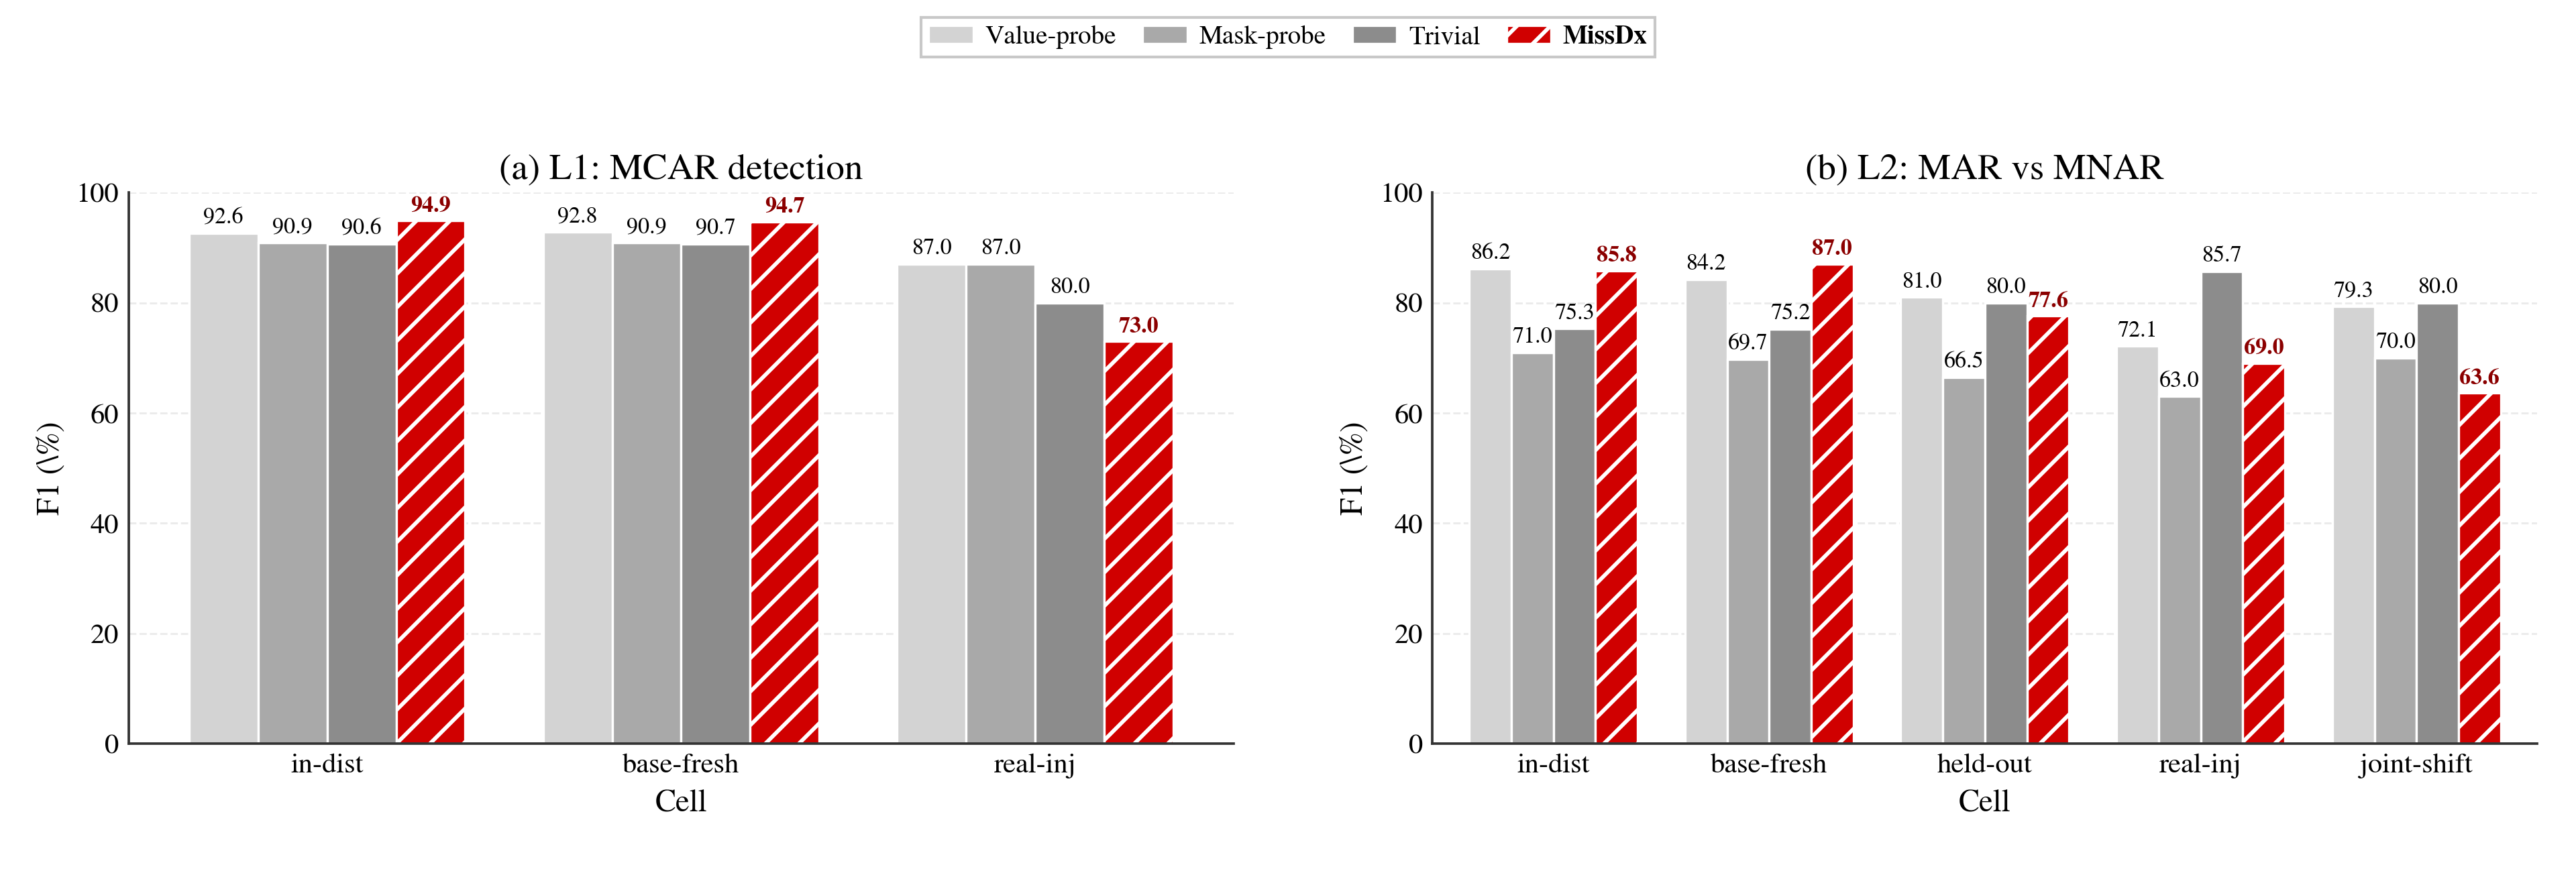
\includegraphics[width=\textwidth]{figs_skill/fig_levels.png}
\caption{Level-structured results in percent (Table~\ref{tab:levels}): (a) L1, MCAR detection F1; (b) L2, MAR-family vs MNAR-family F1. MissDx is hatched; the trivial baseline is gray. Heckit is omitted because it emits no L1 and no in-distribution L2 value.}\label{fig:levels}
\end{figure*}

\subsection{Against Little's Test and the Selection-Model Score Test}\label{sec:little}

\begin{table}[t]
\caption{Per-family recall and precision (from the same in-distribution confusion matrix,
$n{=}900$, 150 per family) and the largest sink: the fraction of the family routed to its most
frequent wrong family. Skip is nearly perfect (deterministic co-occurrence); latent-MNAR, the
theoretical boundary class, is correctly recalled but with the highest posterior entropy.}
\label{tab:perfamily}
\centering\small
\begin{tabular}{lccr}
\toprule
Family & Recall & Precision & Largest sink \\
\midrule
MCAR & .707 & .757 & latent-MNAR .28 \\
MAR-obs & .560 & .712 & self-mask .24 \\
Self-mask & .727 & .712 & MAR-obs .15 \\
Latent-MNAR & .840 & .681 & MCAR .15 \\
Skip & .987 & .993 & MAR-obs .01 \\
Mixture & .767 & .742 & MAR-obs .07 \\
\bottomrule
\end{tabular}
\end{table}

\begin{figure}[t]
\centering
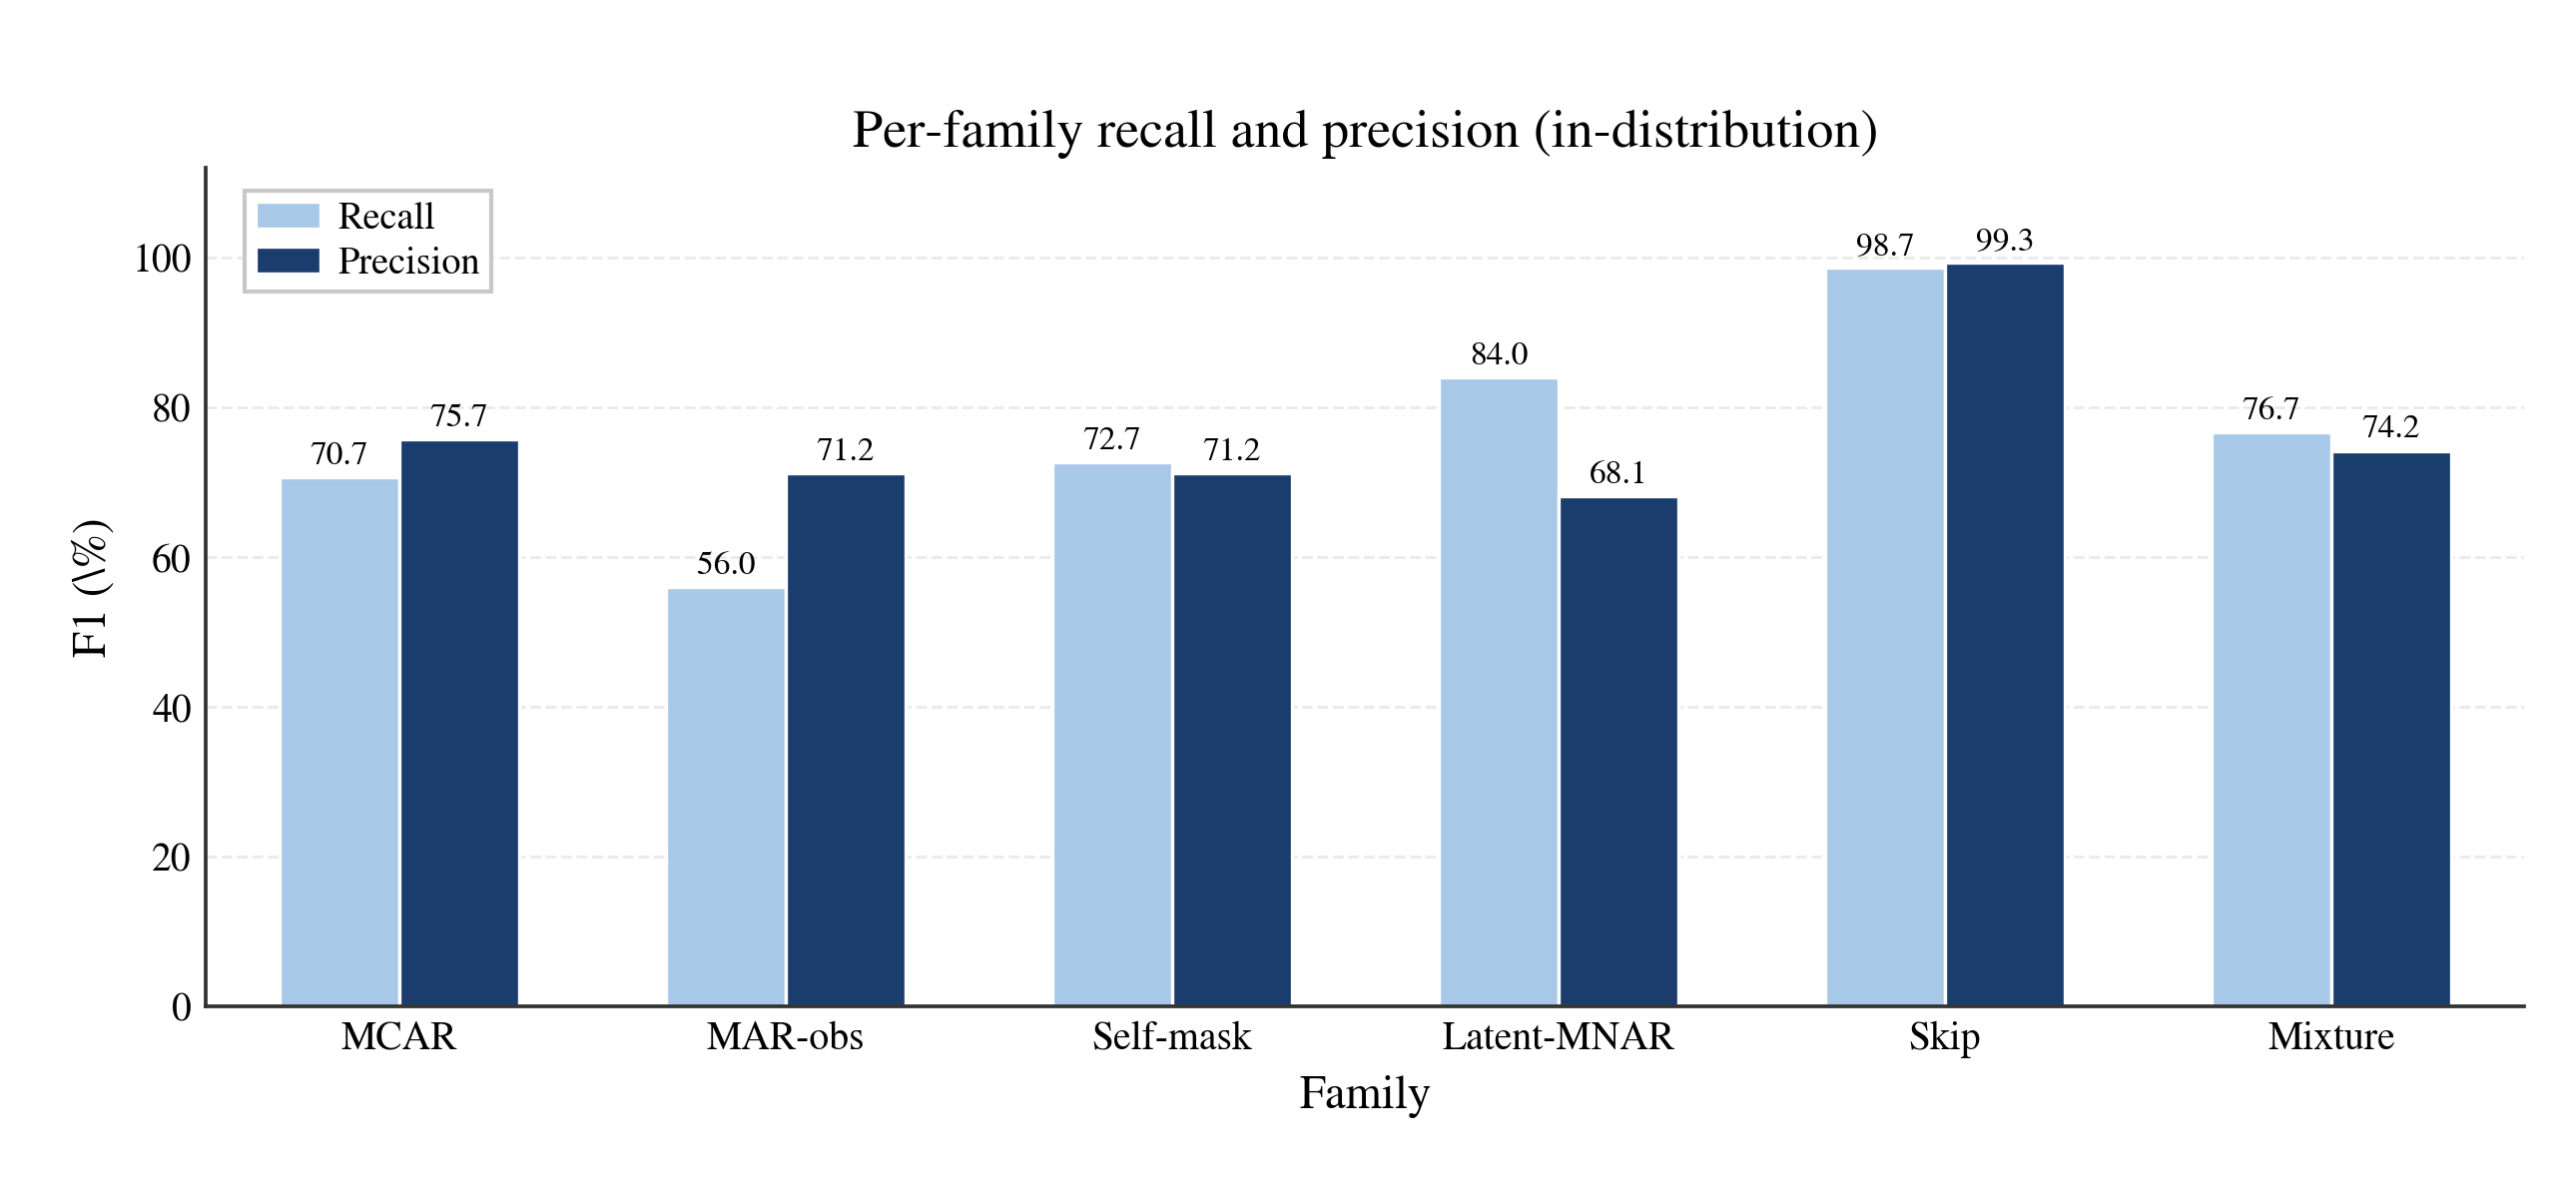
\includegraphics[width=\linewidth]{figs_skill/fig_per_family.png}
\caption{Per-family recall and precision from the in-distribution confusion matrix (Table~\ref{tab:perfamily}), in percent.}\label{fig:perfamily}
\end{figure}

Table~\ref{tab:perfamily} decomposes the in-distribution confusion matrix: skip is nearly
perfect (deterministic categorical co-occurrence is a trivial signal); MCAR and MAR-obs are
the weakest (both rely on the absence of heterogeneity, a weaker signal than its presence);
and latent-MNAR, the theoretical boundary class, achieves high recall but with the highest
posterior entropy among correct predictions (Sect.~\ref{sec:missdx}). The off-diagonal structure
is informative in two ways. First, the two MAR/MNAR confusions are asymmetric at the family
level: self-mask leaks to MAR-obs ($24\%$) more than the reverse ($15\%$), because a
one-covariate selection model is also fit by a self-selection on the correlated driver that
MAR-obs leaves observed. Second, the boundary class's errors fall on MCAR ($15\%$), not on MAR:
when the latent driver carries little residual signal the table looks homogeneous, which is
exactly the collapse that Proposition~\ref{prop:hier}(ii) predicts and the reason its posterior
entropy, not its accuracy, is the quantity we report.

The headline detection result: pooled over base-fresh, held-out and the four-source
real-injected cell on which the detection comparison was run ($n=1{,}092$; 926 non-MCAR, 166
MCAR), MCAR detection gives AUROC $0.948$--$0.954$ for the diagnostic against $0.899$--$0.903$
for a pattern-targeted moment test (per-pattern group means, $\chi^2$ tail): an advantage of
$+4.6$--$5.5$\,pp, with per-seed 95\% paired-bootstrap intervals of $[3.6,7.4]$, $[2.6,6.5]$,
and $[2.8,6.7]$\,pp (three test-pool draws) that exclude zero, and on the small-$n$ stratum
(tables under 600 rows, $n\approx490$) it is $+4.3$--$5.6$\,pp.

We also run the classical parametric alternative end-to-end: a Heckman two-step selection test
(probit selection on covariates, Mills-ratio-augmented outcome regression, $t$-test on the Mills
coefficient, per corrupted column; minimum $p$ across columns), the distributional-prior route of
Remark~\ref{rem:heckman} \cite{heckman1979,dk1994}. Its L2 F1 ranges $0.73$--$0.85$, within
$0.8$--$3.6$\,pp of the majority baseline in every cell and never above it; its accuracy is
within $2.8$\,pp of the constant predictor; and its predicted-MNAR rate ($0.87$--$0.96$) exceeds
the true prevalence ($0.60$--$0.75$), i.e.\ it over-asserts MNAR. Marginal misspecification
predicts this size distortion, though our threshold was tuned on a class-imbalanced subset
and part of the gap is miscalibration, not the test itself. A correctly specified
Gaussian control validates the implementation and localizes the phenomenon: with 150 replicates,
size is controlled (false-positive rate $0.01$--$0.09$ at level $0.05$) and power requires a
predictable component. At $\tau_f^2=0$ power stays at $0.04$--$0.08$ for every $b$ (no
exclusion restriction, Mills collinear with the intercept); at $\tau_f^2=0.49$ it rises from
$0.07$ ($b{=}0.5$) to $0.61$ ($b{=}3$), and at $\tau_f^2=0.66$ it reaches $0.71$; under $t_3$
marginals the false-positive rate inflates to $0.18$. The predictability knob is the same
$\tau_f^2$ as in the attenuation law (Lemma~\ref{lem:esn}). The parametric prior thus neither
rescues the joint-shift cell ($0.778$ vs trivial $0.800$) nor challenges the nonparametric
channel in-family ($0.734$ vs value-probe $0.880$).

\subsection{Theory Validation: the Attenuation Law}\label{sec:exp-validate}

\begin{figure}[t]
\centering
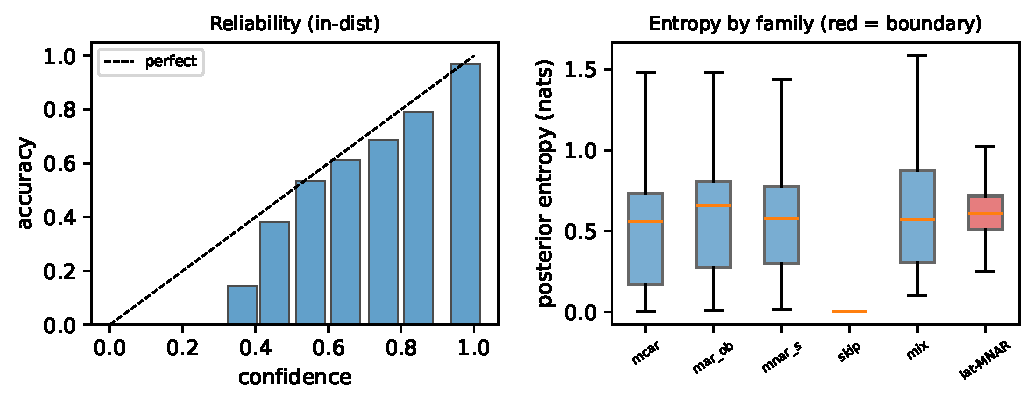
\includegraphics[width=\linewidth]{figs/fig_calib.pdf}
\caption{Left: reliability diagram on the in-distribution pool (ECE $0.033$). Right:
posterior entropy by family. The boundary class (latent MNAR, red) has the highest median
entropy, consistent with the theory that its signal is weakest.}\label{fig:calib}
\end{figure}

On a controlled Gaussian generator with oracle residuals (unit total variance, $\sigma^2=1-\tau_f^2$), the ESN-predicted skewness tracks the
empirical value over the $(\tau_f^2,b)$ 16-point grid (Fig.~\ref{fig:esn}): median absolute
deviation $0.008$, maximum $0.029$, against a Monte-Carlo standard error of about $0.011$ from
50 replicates per cell. When the fit is re-estimated on observed rows instead of oracle residuals
the deviation rises to $0.28$; the law is a population-oracle statement and we report the gap.
At $b=3$ the predicted skewness attenuates from $0.667$ ($\tau_f^2=0$) to $0.018$
($\tau_f^2=0.81$), a $36\times$ decay along Eq.~\eqref{eq:attenuation}, with empirical (oracle)
endpoints $0.659$ and $0.009$. A supplementary six-cell grid at missingness rate $0.25$
($\alpha_0\ne0$) validates the extended branch against exact ESN-density sampling
(observe-side sign applied): deviations $\le0.033$ in magnitude, matching the $\alpha_0=0$
scale. All 16 main cells sit at $\alpha_0=0$, i.e.\ in the classical
skew-normal sub-case; the extended ($\alpha_0\ne0$) branch is not validated here. The
$\lambda$-sweep (Fig.~\ref{fig:lambda}) shows the mv-channel signal decaying monotonically
($0.375\to0.140$) with model entropy high at both ends (near-independent selection at low
$\lambda$, vanishing signal at $\lambda\to0.95$) and lowest mid-range, where the
self-mask-like signal is strongest. Uncertainty localizes where the observable signal vanishes.

\begin{figure}[t]
\centering
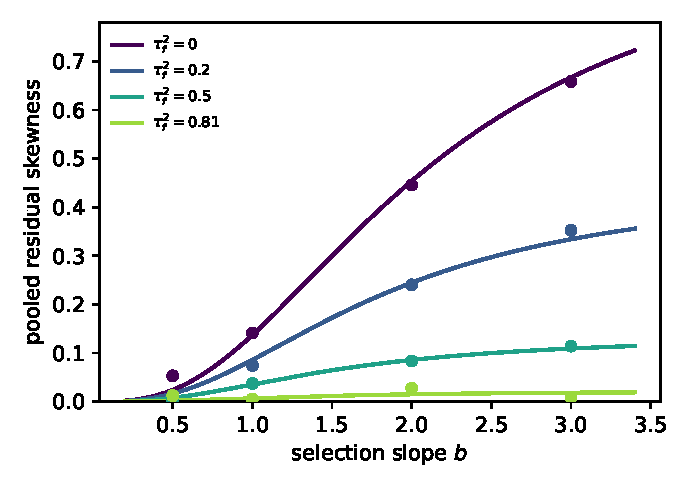
\includegraphics[width=.90\linewidth]{figs/fig_esn.pdf}
\caption{Attenuation law (Lemma~\ref{lem:esn}): predicted skew-normal skewness (lines) vs empirical pooled residual skewness (circles) over $(\tau_f^2,b)$; circles are sign-flipped from the observe side to the missing side. Empirical values use oracle residuals; re-fit residuals deviate from the prediction by up to $0.28$.}\label{fig:esn}
\end{figure}
\begin{figure}[t]
\centering
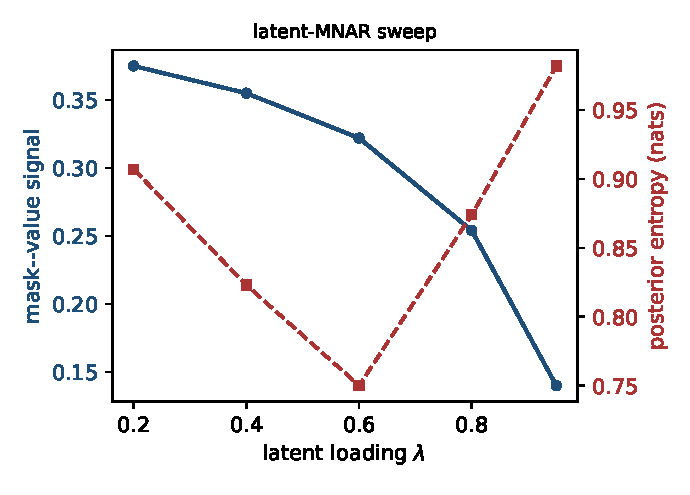
\includegraphics[width=.90\linewidth]{figs/fig_lambda.pdf}
\caption{Latent-MNAR sweep: the mv-channel signal decays monotonically with the latent loading
$\lambda$ while posterior entropy localizes (U-shaped: confident at low $\lambda$, uncertain as
the signal vanishes).}\label{fig:lambda}
\end{figure}

\subsection{Mechanism-to-Treatment Routing: A Preregistered Boundary Measurement}\label{sec:e3b}

\begin{table}[t]
\caption{Treatment-arm values on the routing experiment (180 small tables, $n\le150$ rows,
RandomForest downstream; 30 calibration and 30 test tables per coarse class).
\emph{Top:} prediction accuracy of each fixed policy by true mechanism class, measured on the
calibration pool; the best fixed policy is mean imputation, whose test-pool accuracy is $.618$.
\emph{Bottom:} $\beta$-estimation error (mean absolute deviation of the recovered slope) for the
same policies plus complete-case; under MAR every policy is an order of magnitude worse. Neither
task separates policies: the oracle (per-class best) gains $-0.1$\,pp over blind. The last two
rows of panel (a) are routed test-pool accuracies for the blind (mean-imputation) and oracle
per-class policies.}
\label{tab:vtable}
\centering\small
\begin{tabular}{lcccc}
\toprule
\multicolumn{5}{l}{\emph{(a) Prediction accuracy (calibration pool)}}\\
True class & Mean & $k$-NN & Iter. & Mask-feat \\
\midrule
MCAR & .628 & .625 & .626 & .618 \\
MAR  & .612 & .608 & .613 & .605 \\
MNAR & .621 & .606 & .619 & .621 \\
\midrule
Blind & \multicolumn{4}{c}{.618} \\
Oracle & \multicolumn{4}{c}{.617} \\
\midrule
\multicolumn{5}{l}{\emph{(b) $\beta$-estimation error (lower is better)}}\\
True class & Mean & $k$-NN & Iter. & Compl. \\
\midrule
MCAR & .399 & .395 & .389 & .399 \\
MAR  & 2.069 & 2.057 & 2.058 & 2.069 \\
MNAR & .280 & .261 & .262 & .280 \\
\bottomrule
\end{tabular}
\end{table}

A natural follow-up question for a mechanism diagnostic is whether it selects better
treatments (impute, model, or bound). A preregistered experiment on 180 small-sample tables
($n\le150$ rows, nonlinear downstream) compared five routing policies: blind (best fixed
policy), oracle (sees the true mechanism), MissDx-routed, probe-routed, and Little-routed. The
four treatment arms were mean imputation, $k$-NN, iterative model-based imputation, and
imputation-plus-missingness-indicator features, evaluated on downstream RandomForest
classification accuracy and on $\beta$-estimation bias. Table~\ref{tab:vtable} shows
the policy values by class: the oracle routing gain over blind
is $-0.1$\,pp, i.e.\ the four policies are equivalent even when the true mechanism is known.
The measurement isolates the bottleneck precisely: at the effect sizes and sample sizes our
benchmark covers, standard imputation policies are insensitive to the mechanism, so the
mechanism is not the binding constraint. This is why the routing rule prescribes \texttt{BOUND} and
\texttt{SENSITIVITY\_ANALYSIS} rather than selecting among
imputers; it closes the routing question under our benchmark. The $\beta$-estimation panel
makes the same point from the estimation side: under MAR every policy errs by an order of
magnitude more than under MCAR or MNAR, yet the policies remain indistinguishable from one
another, so no routing decision can help---only bounding or sensitivity analysis can.

\subsection{Feature Ablation}\label{sec:ablation}

Per-column feature importance (zeroing each feature of the value-aware probe and observing the in-distribution macro-F1 drop) shows no dominant channel: the top five columns (indices 25, 14, 2, 6, 27) cost $1.7$, $1.6$, $1.5$, $1.5$, $1.2$\,pp and span the $\phi$ (mask-mask), point-biserial (mask-value), residual-shift, and rate channels. This is consistent with the theory (Prop.~\ref{prop:hier}): multiple testable restrictions must jointly fail before MCAR is rejected, so removing any one channel only mildly degrades detection. The pooled residual-shape channel (skewness and kurtosis of the re-fit residuals) costs only $0.3$\,pp when ablated, exactly what Lemma~\ref{lem:pooled} predicts.

\subsection{Heckit Control: Where Parametric Power Comes From}\label{sec:heckit-control}

The Heckit two-step selection test is correctly specified only when the outcome model is
Gaussian and the selection link probit. Under such a control (150 replicates per cell) size
is controlled (false-positive rate $0.01$--$0.09$ at level $0.05$), and power requires a
predictable component: at $\tau_f^2=0$ it stays at $0.04$--$0.08$ for every $b$; at
$\tau_f^2\approx0.49$ it rises from $0.07$ ($b{=}0.5$) to $0.61$ ($b{=}3$), reaching
$0.71$ at $\tau_f^2\approx0.66$; under $t_3$ marginals the false-positive rate inflates to
$0.18$. The $\tau_f^2$-dependence that Lemma~\ref{lem:esn} predicts, not an implementation
artifact, explains the Heckit's failure on our benchmark (Sect.~\ref{sec:little}).

\subsection{Calibration Under Shift}

Table~\ref{tab:calib_deg} reports the
diagnostic's expected calibration error (ECE) per cell, at both the fine-grained
(6-class) and coarse (3-class) levels. In-distribution calibration is excellent
(ECE $\le0.04$), and the coarse ECE tracks shift severity across the deployment cells:
$0.067$ on held-out mechanism families, $0.223$ on real tables, $0.305$ under joint
shift. Because the posterior reports this degradation instead of hiding it, out-of-domain
deployment is detectable from the diagnostic's own output, which is what triggers the
\texttt{SENSITIVITY\_ANALYSIS} fallback of the routing rule.

\begin{table}[t]
\caption{Calibration degradation (ECE) across evaluation cells. \emph{Dashes}: fine-grained
ECE is undefined for cells whose mechanism labels are outside the six-class training
vocabulary (held-out families and real tables carry labels the posterior never saw).}\label{tab:calib_deg}
\centering\small
\begin{tabular}{lcc}
\toprule
Cell & ECE (fine) & ECE (coarse) \\
\midrule
in-dist & .035 & .041 \\
base-fresh & .019 & .033 \\
held-out & --- & .067 \\
real-inj & --- & .223 \\
joint-shift & --- & .305 \\
\bottomrule
\end{tabular}
\end{table}

\begin{figure}[t]
\centering
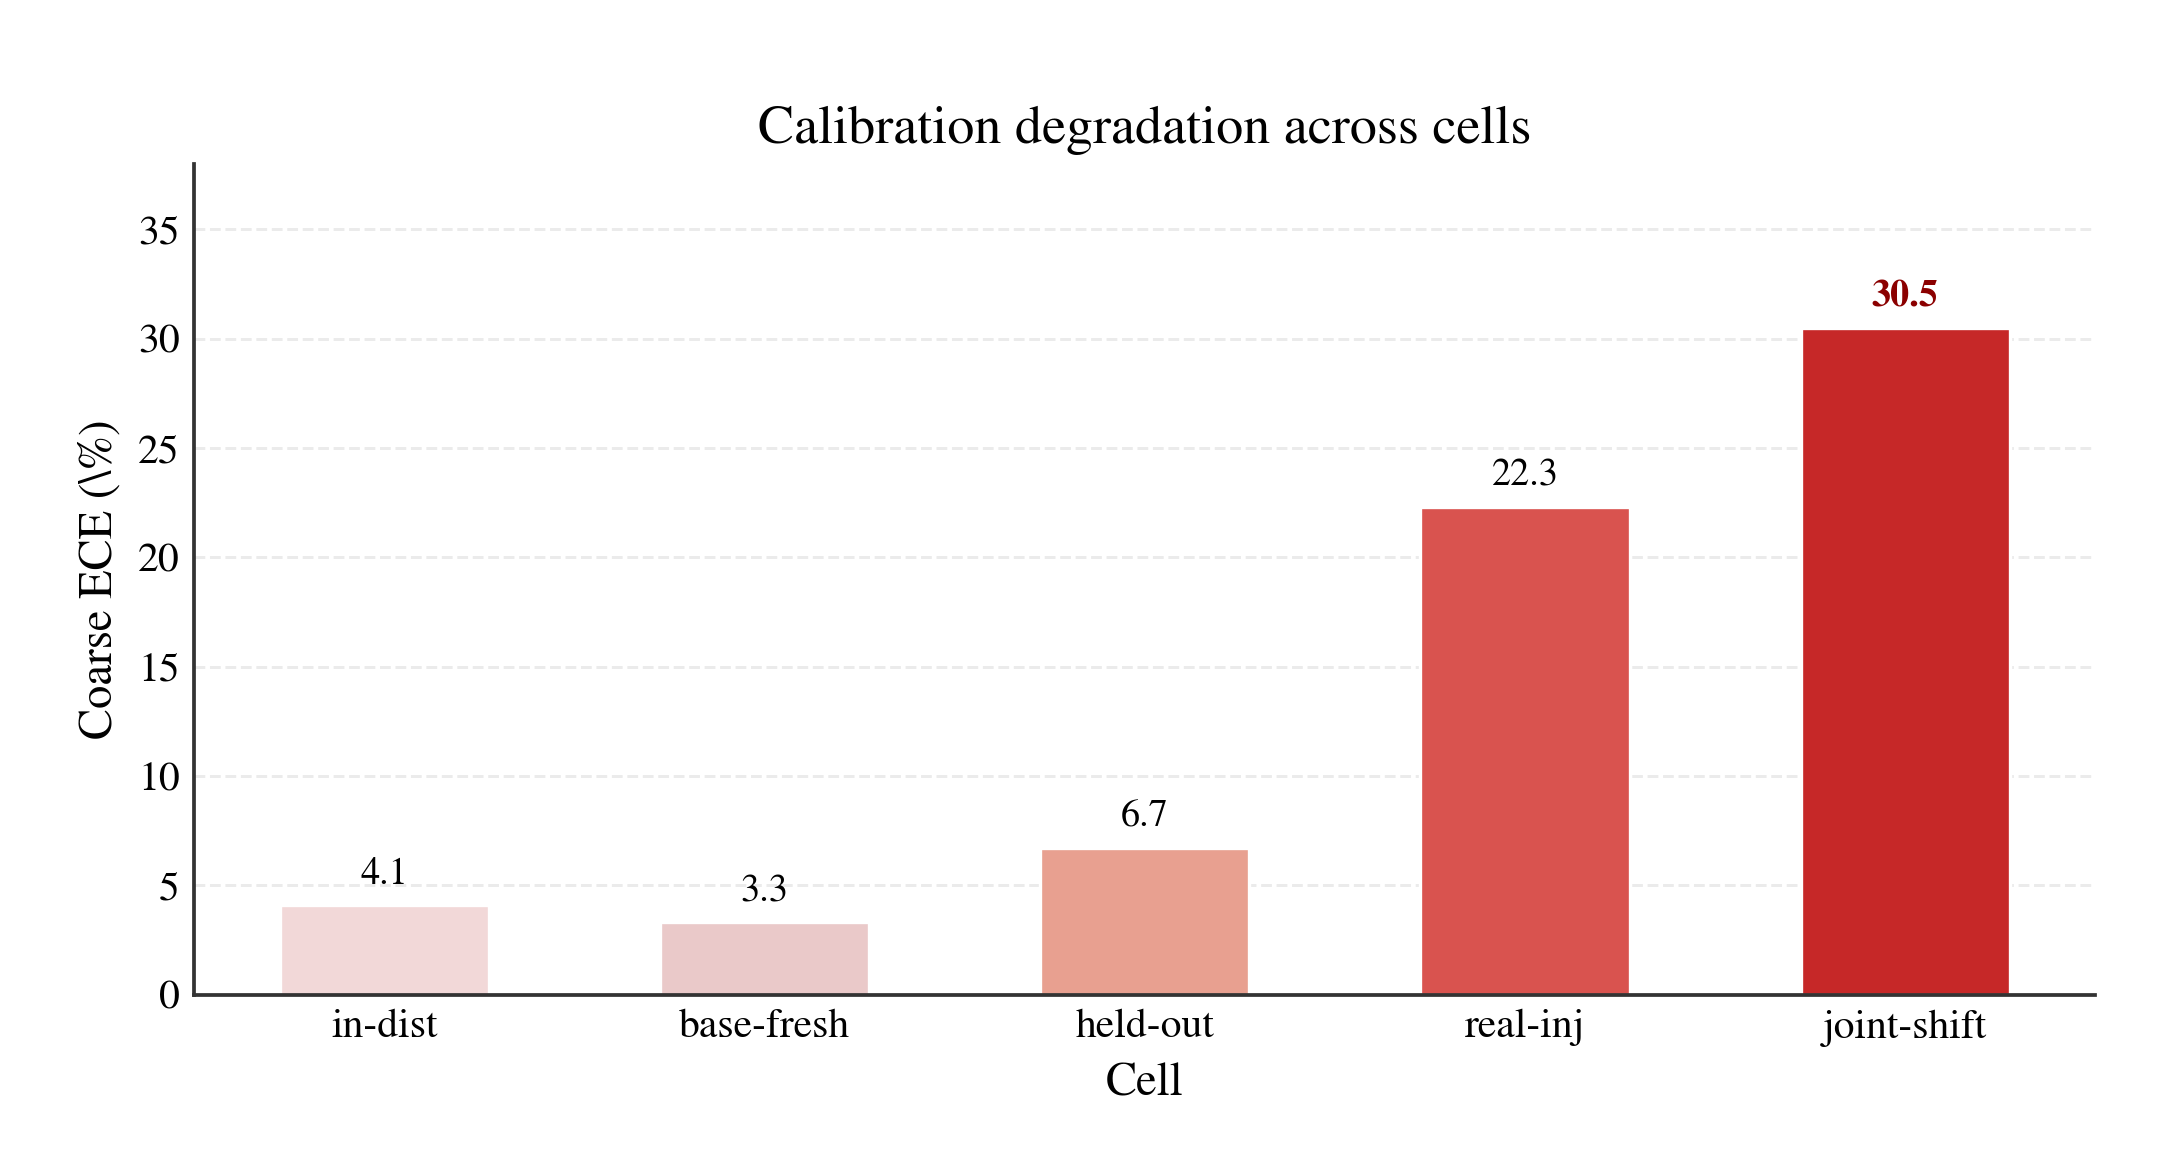
\includegraphics[width=\linewidth]{figs_skill/fig_calib_ece.png}
\caption{Coarse-grained calibration error per cell (Table~\ref{tab:calib_deg}); darker bars mark stronger distribution shift.}\label{fig:calib_ece}
\end{figure}

\subsection{Link-Relative Strength}\label{sec:strength}

With rates calibrated to $25\%$ at the observed driver, the same nominal $b$ yields different
quantile contrasts across links ($b{=}2$: probit $0.970$ vs logit $0.787$); matching a common
contrast $C\approx0.787$ requires probit $b\approx1.19$ vs logit $b=2.0$, a ratio of $1.69$.
The classical $1.7$ rescaling is recovered in a closed-form link calculation. This explains why
strength estimators fail cross-link transfer ($\rho\le0.11$ across links; the strength axis
failed its pre-registered criterion); in-distribution rank correlation reaches only
$\rho\approx0.40$--$0.43$, pooled over base families with different links (partial recovery). Conversely, an observable-projection estimator of the quantile contrast (a probit fit
of missingness on the cross-validated predicted component of the target column) recovers the
invariant functional within families ($\rho\approx0.87$--$0.92$) and transfers partially across
links (pooled $\rho=0.55$ over probit/logit/threshold families, against $\le0.11$ for raw-$b$
estimators). The link-invariant target of Prop.~\ref{prop:link} is estimable in principle,
attenuated by the projection. Practitioners comparing selection strength across tables should
therefore report the contrast $s(q_{90})-s(q_{10})$ estimated on the observable projection,
not a raw coefficient.


\section{Discussion and Limitations}\label{sec:disc}
The theory names the two exits from the single-table impasse: distributional priors (the
selection-model route, with known fragility) or \textbf{external references}, such as multiple
tables sharing mechanisms, historical versions, or instrument-like collection changes. External
references restore a reference for the counterfactual shape. Within a single table,
Remark~\ref{rem:sep} leaves one crumb: \emph{conditional} residual shapes carry the MAR/MNAR
signal; exploiting them requires reliable conditional estimation, i.e.\ strong predictability,
which is exactly what the attenuation law says real tables lack.

Three boundary measurements make the theory operational. First,
mechanism-to-treatment routing: with 30 tables per class for
calibration and test (180 tables), the policy that sees the true mechanism gains nothing over
the blind policy (regret $-0.001$), so the binding constraint at realistic sample sizes is the
insensitivity of the imputation policies, not the diagnosis; the routing rule is designed
accordingly. Second, selective prediction: at posterior confidence $0.9$ the diagnostic
accepts 33--42\% of real tables at an error rate of $0.46$--$0.62$, and its calibration
error rises from $0.035$ (fine-grained, in-distribution) to $0.223$ on real tables and
$0.305$ under the joint shift at the coarse level, where the fine-grained error is undefined
(Sect.~\ref{sec:exp-levels}); the diagnostic therefore reports its own domain, and the
coarse ECE is the signal that triggers the sensitivity-analysis fallback. Third, the learned
aggregator is matched by a linear probe on the same features outside the training families,
so the value of MissDx lies in its calibrated uncertainty and declared domain, not in the
representation. What the theory supports
is therefore a \emph{calibrated mechanism-risk warning} consumed by a sensitivity analysis,
not an autonomous routing decision---and MechZoo is the instrument that turns each of these
statements into a reproducible measurement. Table~\ref{tab:per-source} decomposes the
real-table cell by source: the aggregate is not an artifact of one table but varies widely,
and the diagnostic wins on five of the nine sources, a consequence of the
\emph{size} of the losses, not their number. We therefore treat the real cell as nine
correlated replications rather than 432 independent tables.

\begin{table}[t]
\caption{Per-source L2 (MAR-family vs MNAR-family) coarse-F1 of the diagnostic and the
value-aware linear probe on the real-injected cell; each source contributes 48 injected
tables. $\Delta$ is MissDx minus probe. Note that per-source and pooled F1 are \emph{not} a
weighted average of one another: L2 excludes MCAR-labelled tables, so each source contributes a
different subset to each figure.}
\label{tab:per-source}
\centering\small
\begin{tabular}{lccc}
\toprule
Source & MissDx & Value-probe & $\Delta$ \\
\midrule
breast-cancer & .631 & .513 & $+$.118 \\
diabetes & .413 & .632 & $-$.219 \\
page-blocks & .370 & .333 & $+$.037 \\
MagicTelescope & .724 & .777 & $-$.053 \\
balancing-scale & .478 & .375 & $+$.103 \\
qsar-biodeg & .455 & .472 & $-$.017 \\
wine-quality-white & .483 & .095 & $+$.388 \\
synthetic-control & .449 & .295 & $+$.154 \\
ILPD & .554 & .656 & $-$.102 \\
\midrule
pooled & .690 & .721 & $-$.031 \\
\bottomrule
\end{tabular}
\end{table}

\begin{figure*}[t]
\centering
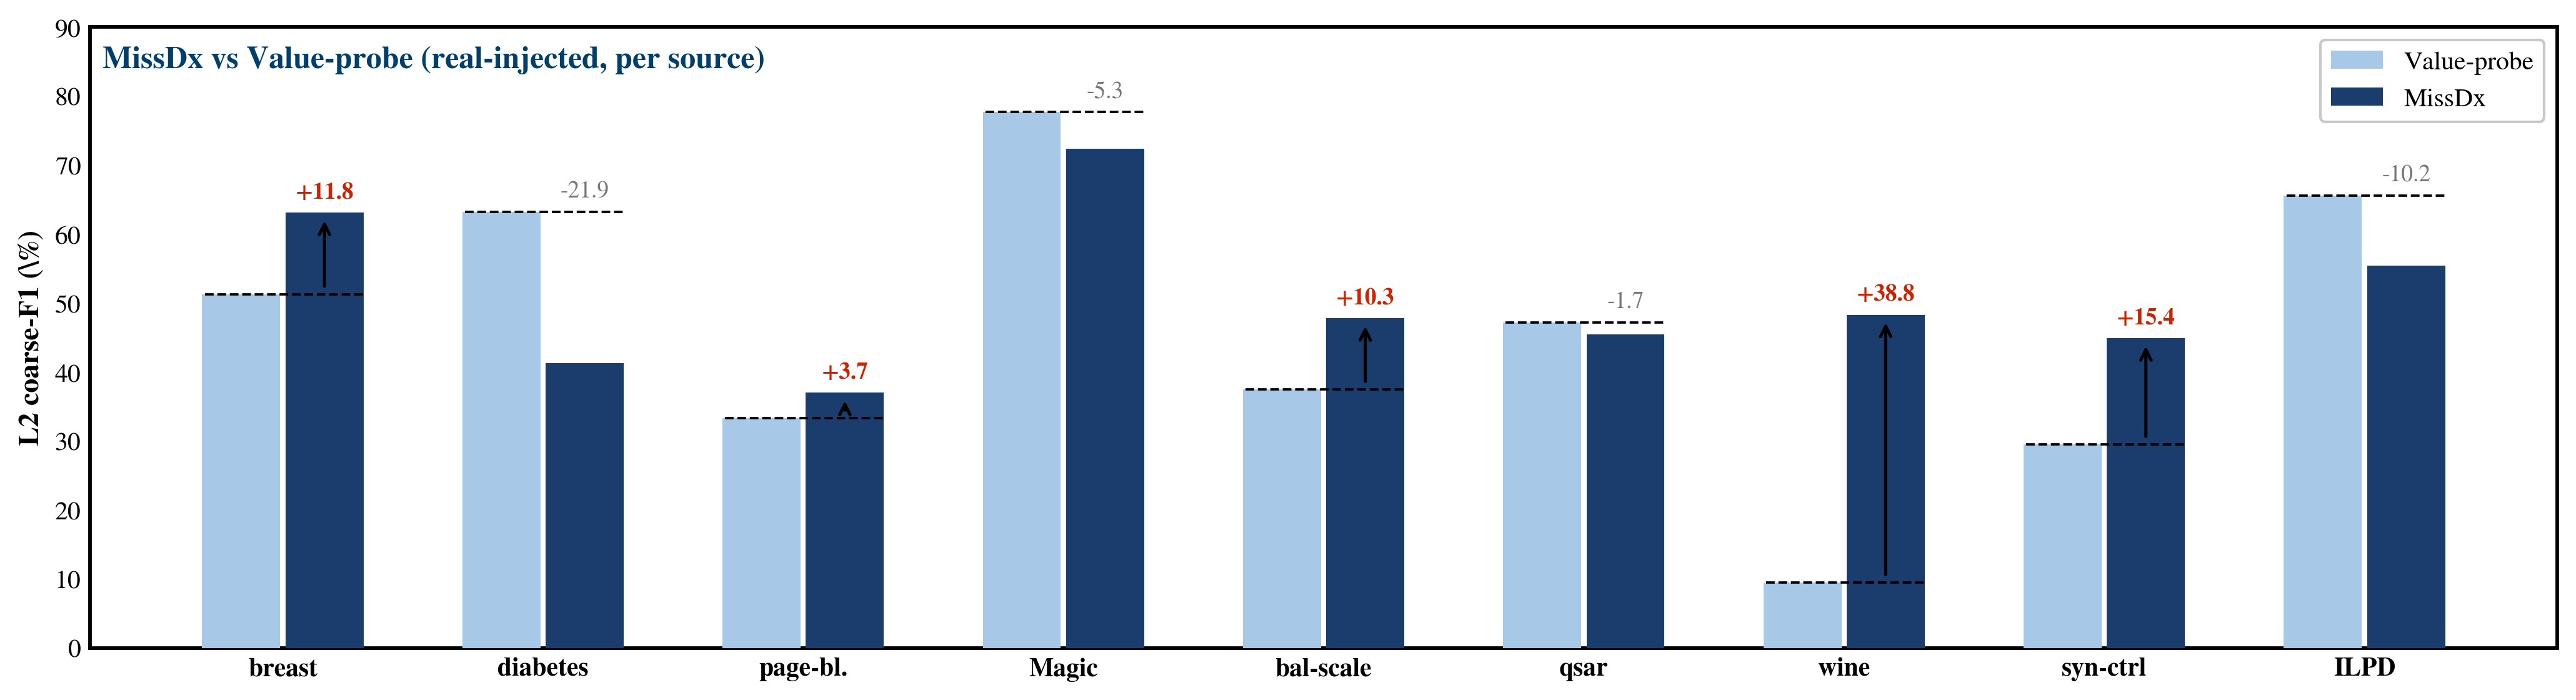
\includegraphics[width=\textwidth]{figs_skill/fig_per_source.png}
\caption{Per-source L2 coarse-F1 on the real-injected cell (Table~\ref{tab:per-source}): MissDx against the value-aware probe, with the per-source gap in percentage points.}\label{fig:per_source}
\end{figure*}

Limitations: the diagnostic accepts numeric columns only and at most 12 of them; the benchmark
covers 2{,}472 tables of at most 1{,}000 rows, and its real side is nine public tables with
injected mechanisms, so no claim here is about naturally occurring missingness; held-out families
shift the functional form, driver structure and shape of the mechanism, not its semantics
(limit-of-detection censoring, designed skips in survey instruments, item nonresponse).
External-reference mechanism identification remains the open problem; recovery-sample designs
\cite{noonan2022} and shadow variables are the existing partial answers.

\paragraph{From theory to action.} The theory yields a per-column routing rule. \emph{L1}
is the only guaranteed verdict: homogeneous or drifting, with the drifting columns and
patterns identified (Prop.~\ref{prop:hier}). \emph{L2} is a posterior over mechanism
families, valid only within its declared calibration domain; $\hat\tau_f^2$ is the trust
knob (high predictability makes detection possible, low calls for a sensitivity analysis,
Lemma~\ref{lem:esn}); $\hat C$ is a link-invariant strength contrast
(Prop.~\ref{prop:link}). The routing follows: \texttt{IMPUTE} when L1 reports homogeneity,
\texttt{SENSITIVITY\_ANALYSIS} when the posterior is flat or the table leaves the
calibration domain, and \texttt{BOUND} in between, returning
$[\hat x_j^{\mathrm{MAR}}, \hat x_j^{\mathrm{MAR}}\times(1+\hat C)]$. Three consequences
follow. (1)~\emph{MCAR screening is safe, localizable, and robust}: the homogeneity layer is
testable, points to the drifting columns and patterns, and is stable across tables and
deployable at any scale; our diagnostic improves its AUROC over Little's test by
$+4.6$--$5.5$\,pp. (2)~\emph{Single-table MAR/MNAR labels are not trustworthy}: the theory
proves this, and the joint-shift cell confirms it for every system we evaluated, so the
defensible output is a bounded warning---``self-selection detected/not excluded, confidence
domain: generator family X''---rather than a definitive label. (3)~\emph{The cross-column
predictability $\tau_f^2$ is the one statistic to track}: the attenuation law
(Lemma~\ref{lem:esn}) and the Heckit control both point to it, and a per-column report of
$\hat\tau_f^2$ says immediately whether mechanism diagnosis is worth attempting. Per-column
features cost $O(nd^2)$ ($\sim$15\,ms per column at our benchmark sizes), so the rule is cheap
to run.

\paragraph{Future directions.} Three extensions follow from the theory. (1)~\emph{Corpus-level
diagnosis}: tables that share a mechanism---common in data lakes and versioned
datasets---restore the identifiability a single table lacks (Lemma~\ref{lem:dual}) by serving
as external references; an amortized diagnostic that pools evidence across tables, conditioned
on table metadata, is the natural next step. (2)~\emph{Mixed-type columns}: our features cover
numeric columns only; extending the cross-prediction residual to categorical targets would
cover the structurally driven skips that real survey tables carry. (3)~\emph{Incremental
diagnosis}: the per-column features update in $O(d)$ per arriving row, so the diagnosis can be
maintained as a table grows.

\paragraph{Sensitivity analysis as fallback.} When the rule outputs
\texttt{SENSITIVITY\_ANALYSIS}, the practitioner replaces point imputation with a
$\delta$-adjusted analysis: impute under MAR, then scale each imputed value by a sensitivity
parameter $\delta\in[0.9,1.1]$ (or shift it by $\pm\Delta$) and re-estimate the downstream
quantity for each $\delta$. The resulting tipping-point curve shows how far the departure
from MAR must go before the conclusion flips. The theory guarantees this is the correct
fallback: Lemma~\ref{lem:dual} shows a single table cannot distinguish MAR from MNAR, so the
answer is a range, not a point. The reported $\hat\tau_f^2$ sets a data-driven default for
$\Delta$: high $\hat\tau_f^2$ means a small likely MNAR departure, low $\hat\tau_f^2$ calls
for a wider range.

\paragraph{Summary of boundary results.} Table~\ref{tab:negatives} lists all four
preregistered boundary findings, their criteria, and their status. Each one sharpens the
boundary of what a single-table diagnostic can claim, and the theory explains each one.

\begin{table}[t]
\caption{Preregistered boundary results. All criteria were set before the experiment was
run; none was modified after seeing the data.}
\label{tab:negatives}
\centering\small
\begin{tabular}{@{}llll@{}}
\toprule
Boundary & Criterion & Result & Expl. \\
\midrule
Routing & oracle$\ge$3pp & $-0.1$pp & insens. \\
Strength & $\rho\ge.40$ & $\le.11$ & Prop.~2 \\
Pooled & $+5$pp & $+0.3$ & Lem.~3 \\
Calib. & ECE$\le.10$ & .22 & o.o.d. \\
\bottomrule
\end{tabular}
\end{table}

\paragraph{Threats to validity.}
\emph{Internal:} our per-column features are computed by a single procedure; alternative
featurizations could change the level-1/level-2 split. The three test-pool draws use a
fixed model checkpoint; training variance is bounded by the $0.4$\,pp gap between
our two training runs. Cluster-level
inference on the real-table cells treats the nine source tables as clusters of 48
near-replicates, and we state this explicitly wherever those intervals are reported. \emph{External:} MechZoo
covers synthetic mechanisms with calibrated rates on $\le$12 numeric columns; coverage of
mixed-type tables, wider column sets, and naturally occurring missingness (as opposed to
injection) remains open. The held-out families shift functional form and driver structure
but not semantic mechanism types (limit-of-detection censoring, designed survey skips,
item nonresponse). \emph{Construct:} our L2 metric pools three MNAR sub-families against
two MAR sub-families; the prevalence ratio (2:1 or 3:1) directly determines the majority
baseline, so L2 absolute values should be read relative to that baseline, not in
isolation.

Table~\ref{tab:theory-exp} interlocks theory and experiment: every theoretical result has an
empirical counterpart.

\begin{table}[t]
\caption{Theory--experiment interlock: each theoretical result and its empirical counterpart.}
\label{tab:theory-exp}
\centering\small
\begin{tabular}{@{}p{0.62in}p{2.63in}@{}}
\toprule
Result & Empirical counterpart \\
\midrule
Prop.~\ref{prop:hier}(i) & MCAR $\Rightarrow$ homogeneity; detection vs Little (Sect.~\ref{sec:little}): AUROC $.95$ vs $.90$. \\
Prop.~\ref{prop:hier}(ii) & homogeneity is the only non-trivial restriction; hierarchy table (Table~\ref{tab:levels}): L1 clears the baseline, L2 collapses. \\
Lemma~\ref{lem:dual} & MAR/MNAR dual rationalization; joint-shift cell (Table~\ref{tab:levels}): every system at or below the majority baseline. \\
Lemma~\ref{lem:esn} & ESN attenuation $\alpha_1=b/\sqrt{1+b^2\tau_f^2}$; 16-cell grid (Fig.~\ref{fig:esn}): median deviation $.008$. \\
Lemma~\ref{lem:pooled} & pooled shape tests cannot be consistent; shape-channel ablation (Sect.~\ref{sec:ablation}): $0.3$\,pp. \\
Prop.~\ref{prop:link} & $b$ link-relative, $C$ link-invariant; strength transfer (Sect.~\ref{sec:strength}): $\rho_C{=}.55$, $\rho_b{\le}.11$. \\
\bottomrule
\end{tabular}
\end{table}

\section{Proofs and Constructions}
\label{sec:proofs}

\paragraph{Lemma~\ref{lem:dual} (MAR side).}
The idea is to build a joint distribution whose \emph{shared-coordinate backbone} is the sum
of the two pattern sub-distributions' shared marginals, then read off MAR selections from
the density ratios. Let
\begin{equation}
\lambda_S=\tilde\mu^0_S+\tilde\mu^1_S,\qquad
h_k=\frac{d\tilde\mu^k_S}{d\lambda_S},\qquad
\gamma^k=\frac{d\tilde\mu^k}{h_k},
\label{eq:proof_mar_defs}
\end{equation}
so that $h_0+h_1=1$ ($\lambda_S$-a.e.), $h_k\in[0,1]$, $h_k>0$ $\tilde\mu^k_S$-a.e., and
$\gamma^k$ is a distribution whose $S$-marginal is exactly $\lambda_S$. Generate $P_X$ by
$x_S\sim\lambda_S$ and the two sides conditionally independently through
$\gamma^k(\cdot|x_S)$; set $s_k(x)=h_k(x_S)$. Then
\begin{equation}
P\bigl(X_{\mathrm{obs}(m^k)}\in dx,\; M=m^k\bigr)
= h_k\,\gamma^k(dx) = \tilde\mu^k(dx).
\label{eq:proof_mar_verify}
\end{equation}
Degenerate cases $S=\emptyset$ (constant selections) and $A_0=A_1$ behave identically.

\paragraph{Lemma~\ref{lem:dual} (MNAR side).}
The idea is to construct a \emph{tilted} completion whose selection probability depends
on the coordinate that is \emph{missing} under $m^0$ ($x_2$). With a bounded jointly
measurable Markov kernel $\rho(x_2|x_1)\le\bar C$ that is non-singular
($m(x_1)=\int\rho\,d\tilde\mu^1(x_1,\cdot)>0$ on $\{\tilde\mu^0>0\}$) and non-degenerate,
define
\begin{equation}
\varphi=\frac{\tilde\mu^0(x_1)\,\rho(x_2|x_1)}{m(x_1)},\qquad
g=\frac{\varphi}{1+\varphi},\qquad
p'=\tilde\mu^1(1+\varphi),
\label{eq:proof_mnar_defs}
\end{equation}
with $\varphi:=0$ where $\tilde\mu^0=0$. Then:
\begin{align}
\text{(i)}\quad \iint p' &= q^1 + \int\tilde\mu^0 = q^1+q^0 = 1; \label{eq:proof_mnar_i}\\
\text{(ii)}\quad p'(1-g) &= \tilde\mu^1 \quad\text{pointwise}; \label{eq:proof_mnar_ii}\\
\text{(iii)}\quad \int p'g\,dx_2 &= \int\varphi\,\tilde\mu^1\,dx_2 = \tilde\mu^0(x_1); \label{eq:proof_mnar_iii}
\end{align}
(iv) $s^0=g$ depends on $x_2$ (missing under $m^0$; non-degeneracy and
$p'\ge\tilde\mu^1$ give mutual absolute continuity per fibre), hence genuinely MNAR;
$s^1=1-g$ depends on $(x_1,x_2)$, both observed under $m^1$.
The assumption class is never empty: the fixed kernel $\rho\equiv\varphi_{N(0,1)}$
satisfies all conditions on every positive-mass fibre.

\paragraph{Proposition~\ref{prop:hier}.}
(i) is immediate from $M\perp X$; the converse fails by the two-pattern construction of
Lemma~\ref{lem:dual} (MNAR side with $\tilde\mu^0$ absorbed into a common $Q$).
(ii) For two patterns, Lemma~\ref{lem:dual} supplies the MAR rationalization and, under
the stated support condition, the genuinely-MNAR twin, so genuine MAR-dependence imposes
nothing on the observed law; heterogeneity is its only non-trivial negation. The
multi-pattern extension requires solving the pointwise constraint
\begin{equation}
\sum_m s_m\bigl(x_{\mathrm{obs}(m)}(x)\bigr)=1 \quad \text{for all } x,
\label{eq:proof_multipattern}
\end{equation}
which is the classical MAR-compatibility statement \cite{rubin1976,mk2007}; we cite it
and do not reprove it, and no result below depends on it.
(iii) follows from Lemma~\ref{lem:dual}: at a genuinely-MNAR point with an MAR twin,
every statistic shares a distribution, so every level-$\alpha$ test of an MAR-containing
null has rejection probability $\le\alpha$ there.

\paragraph{Lemma~\ref{lem:esn}: idea.}
The idea is to compute the pooled weight $w(r)$ in closed form by applying the probit
identity $\mathbb{E}[\Phi(m+sZ)]=\Phi(m/\sqrt{1+s^2})$ to the conditional expectation over
the predictable component $f(X_{-j})$. The result is that the pooled observed-residual
density is an extended skew-normal (ESN) whose slant parameter $\alpha_1$ encodes the
selection strength, attenuated by the predictable variance $\tau_f^2$.
By the probit identity
\begin{equation}
\mathbb{E}[\Phi(m+sZ)]=\Phi\!\left(\frac{m}{\sqrt{1+s^2}}\right),\qquad Z\sim N(0,1),
\label{eq:probit_identity}
\end{equation}
applied conditionally on $\varepsilon=r$:
\begin{equation}
w(r)=\mathbb{E}_{X_{-j}}\bigl[\Phi(a+b(f(X_{-j})+r))\bigr]
=\Phi(\alpha_0+\alpha_1 r),
\label{eq:pooled_weight}
\end{equation}
with $\alpha_1,\alpha_0$ as in \eqref{eq:attenuation} (observe side:
replace $a,b$ by their negation). The pooled density is $f_\varepsilon(r)w(r)/Z$ with the same
identity giving
\begin{equation}
Z=\Phi\!\left(\frac{\alpha_0}{\sqrt{1+\alpha_1^2\sigma^2}}\right).
\label{eq:proof_norm_const}
\end{equation}
Matching against the ESN density
\begin{equation}
\frac{\varphi\bigl((x-\xi)/\omega\bigr)\,\Phi\bigl(\tau+\alpha(x-\xi)/\omega\bigr)}
{\omega\,\Phi\bigl(\tau/\sqrt{1+\alpha^2}\bigr)}
\label{eq:proof_esn_density}
\end{equation}
yields $(\xi,\omega,\alpha,\tau)=(0,\sigma,\alpha_1\sigma,\alpha_0)$. At $\alpha_0=0$ this is
the classical skew-normal, whose skewness is an odd function of the slant with the sign of
$\alpha$ \cite{azzalini2013}.

\paragraph{Lemma~\ref{lem:pooled}.}
Under the MAR generator \eqref{eq:mar_generator}, the selection indicator is
$\sigma(U,X_{-j})$-measurable (with $U\sim\mathrm{Unif}(0,1)$ the selection randomizer),
hence still independent of $\varepsilon'$ conditionally on $X_{-j}$:
\begin{equation}
\mathbb{E}\bigl[X_j \mid X_{-j},\ \text{selected}\bigr] = f(X_{-j}).
\label{eq:proof_cond_mean}
\end{equation}
The population re-fit therefore recovers $f$ up to a constant, and the pooled re-fit
residual law is $q^\ast$ centered, identical to the self-selection side by the
definition of $q^\ast$. Any location-invariant functional
\begin{equation}
T(F) = T(F * \delta_c)\quad \text{for all translations } c
\label{eq:proof_loc_inv}
\end{equation}
therefore agrees on the pair, and so does the probability limit of any statistic
continuous in the residual law.

\paragraph{Remark 1 (separability).}
The idea is that within the ESN family, translations change only the location parameter
$\xi$, preserving the shape parameters. The selected conditional density is
\begin{equation}
\mathrm{ESN}\bigl(f(t),\;\sigma,\;b\sigma,\;a+bf(t)\bigr).
\label{eq:proof_selected_esn}
\end{equation}
Within the family, a translation by $\delta$ maps
$\mathrm{ESN}(\xi,\omega,\alpha,\tau)\to\mathrm{ESN}(\xi+\delta,\omega,\alpha,\tau)$
(the normalization constant is translation-invariant). For $\alpha\ne0$, the parameter
$\tau$ is identified: equality of two such densities forces, by differentiating the
log-ratio,
\begin{equation}
\lambda(\tau_1+u)=\lambda(\tau_2+u)\quad\forall\,u,\qquad
\lambda=\frac{\varphi}{\Phi}\ \text{(strictly decreasing)},
\label{eq:proof_mills}
\end{equation}
hence $\tau_1=\tau_2$. Consequently, if the family were a location family, any two members
would be mutual translations forcing $a+bf(t_1)=a+bf(t_2)$; with $b\ne0$ this means $f$
is constant on the selected support.

\paragraph{Proposition~\ref{prop:link}.}
The idea is a substitution. If $g(a_1+b_1x)=\tilde g(\tilde a+\tilde b x)$ for all
$x\in\mathbb{R}$ with both links strictly increasing, then substituting $t=a_1+b_1x$
yields $\tilde g = g\circ A$ for the affine map
\begin{equation}
A(t)=\frac{\tilde b}{b_1}\,t+\Bigl(\tilde a-\frac{\tilde b}{b_1}\,a_1\Bigr),
\label{eq:proof_affine}
\end{equation}
so exact matches arise precisely within affine classes. For bounded probability links,
no exact cross-link match exists (an affine self-composition of a bounded link that is
exact on all of $\mathbb{R}$ forces the link to be of exponential type, hence unbounded,
a contradiction). Probit/logit achieve the minimax scale $1.702$ with maximum CDF gap
$0.0095$ \cite{haley1952,amemiya1981}. Threshold links identify only $-a/b$.

\paragraph{Edge cases and limitations of the proofs.}
(1)~\emph{Multi-pattern extension}: Lemma~\ref{lem:dual} covers the two-pattern case
(monotone dropout). The multi-pattern extension requires solving the pointwise constraint
$\sum_m s_m(x_{\mathrm{obs}(m)}(x))=1$ across patterns with different observed-coordinate
sets; this is handled by classical MAR-compatibility results
\cite{rubin1976,mk2007,seaman2013}, which we cite without reprove. No result in the main
text depends on the multi-pattern case. (2)~\emph{Gaussianity in Lemma~\ref{lem:esn}}:
the probit identity requires $f(X_{-j})$ to be Gaussian; for non-Gaussian predictable
components the weight $w(r)$ is a convolution smoothing without closed form. The
attenuation law ($\alpha_1\to0$ as $\tau_f^2\to\infty$) is proved only in the Gaussian
case; its qualitative extension to non-Gaussian $f(X_{-j})$ is empirically supported
(the $\lambda$-sweep, Fig.~\ref{fig:lambda}) but not formally established.
(3)~\emph{Degenerate cases in the MNAR construction}: when $f$ is constant on the
selected support (the ``or $f$ degenerate'' exclusion in Remark~1), the MNAR conditional
family collapses to a location family and becomes indistinguishable from the MAR side.
This is a genuine boundary, not a proof gap: the separation result is sharp.
(4)~\emph{Bounded Markov kernel in Lemma~\ref{lem:dual}}: the kernel $\rho$ must be
bounded ($\rho\le\bar C$) and non-singular ($m(x_1)>0$ where $\tilde\mu^0>0$). Unbounded
kernels can make $m(x_1)=\infty$ (the construction degenerates); singular kernels violate
support domination. The assumption class is non-empty (fixed Gaussian kernel works) but
does not cover all possible completions.

\paragraph{Reproducibility.} All code, seeds, and per-table result files are scripted. The
training pool is drawn with seed~$11$ ($24{,}000$ tables), the probes with seed~$21$, and the
five cells with seeds $999$, $777$, $778$, $500{+}k$ (real-injected, source index $k$) and
$900{+}k$ (joint shift, four of the nine sources); per-table model scores and labels are saved
for every cell, so any table-level statistic in this paper can be recomputed without a GPU.
Training the diagnostic takes $190$\,s on one consumer GPU; feature extraction takes about
$15$\,ms per column on a laptop CPU, and the real tables are cached so that the real cells do
not require network access. The generator, all nine mechanism families, the five cells, the
diagnostic checkpoint, the three probes, the Heckit implementation, and every figure and table
script reproduce end-to-end from the released code at
\texttt{https://github.com/REPLACE-ORG/MechZoo} (also given in the submission form).

\section{Conclusion}
A single incomplete table supports exactly one non-trivial mechanism question---pattern
homogeneity---and this paper delivers the complete answer to that question plus a precise
account of where the answer ends. The testable hierarchy (Prop.~\ref{prop:hier}), the dual
rationalization (Lemma~\ref{lem:dual}), and the exact ESN imprint with its validated
attenuation law (Lemma~\ref{lem:esn}) characterize the observable channel exactly: above
homogeneity the MAR/MNAR distinction is generator-class-bound, selection strength is
link-relative, and pooled residual shapes cannot yield a consistent test
(Lemma~\ref{lem:pooled}). On this theory we build three artifacts. MechZoo turns the
boundary into a reproducible measurement under controlled shift. MissDx beats the classical
moment test on the testable level ($+4.6$--$5.5$\,pp AUROC), is calibrated in-distribution,
and reports---rather than hides---where its calibration ends, which is exactly the
information a practitioner needs before trusting a mechanism label. Both are packaged into a single per-column routing rule (impute, bound, or sensitivity
analysis) whose validity conditions are the theorem statements themselves. Together they replace an
unanswerable question (``which mechanism is it?'') with answerable ones: what this table can
tell, and when to fall back to a sensitivity analysis.

\paragraph{Broader impact.} For the data-management community, the practical takeaway is
a \emph{division of labour}: single-table homogeneity screening is safe, useful, and
scalable. It belongs in every data-quality toolkit; mechanism labelling beyond that level
requires external references or distributional assumptions whose cost our theory makes
explicit. The MechZoo fixtures are a step toward
standardized mechanism-diagnosis evaluation; we release them with all code, seeds,
and result files.

\section*{Acknowledgments}
\paragraph{AI-generated content disclosure.} Large language model assistants were used to
help draft and edit prose and to implement, run, and summarise part of the experiments
reported in this paper; every number in the paper is produced by the released scripts, and
the authors are responsible for the correctness and originality of the content.

\bibliographystyle{IEEEtran}

\begin{thebibliography}{25}\small
\bibitem{holoclean2017} I. Rekatsinas, X. Chu, I. F. Ilyas, and C. R\'e, ``HoloClean: Holistic data repairs with probabilistic inference,'' \emph{Proc. VLDB Endow.}, vol.~10, no.~11, pp. 1190--1201, 2017.
\bibitem{rubin1976} D. B. Rubin, ``Inference and missing data,'' \emph{Biometrika}, vol.~63, no.~3, pp. 581--592, 1976.
\bibitem{little1988} R. J. A. Little, ``A test of missing completely at random for multivariate data with missing values,'' \emph{J. Amer. Stat. Assoc.}, vol.~83, no.~404, pp. 1198--1202, 1988.
\bibitem{heckman1979} J. J. Heckman, ``Sample selection bias as a specification error,'' \emph{Econometrica}, vol.~47, no.~1, pp. 153--161, 1979.
\bibitem{dk1994} P. Diggle and M. G. Kenward, ``Informative drop-out in longitudinal data analysis,'' \emph{J. Royal Stat. Soc. C}, vol.~43, no.~1, pp. 49--93, 1994.
\bibitem{seaman2013} S. R. Seaman, J. Galati, D. Jackson, and J. B. Carlin, ``What is meant by `missing at random'?" \emph{Stat. Sci.}, vol.~28, no.~2, pp. 257--268, 2013.
\bibitem{mk2007} G. Molenberghs and M. G. Kenward, \emph{Missing Data in Clinical Studies}. Chichester, UK: Wiley, 2007.
\bibitem{mohanpearl2021} K. Mohan and J. Pearl, ``Graphical models for processing missing data,'' \emph{J. Amer. Stat. Assoc.}, vol.~116, no.~534, pp. 1023--1037, 2021.
\bibitem{noonan2022} J. Noonan, A. A. Adediran, R. Mitra, and S. Biedermann, ``An integrated approach to test for missing not at random,'' \emph{arXiv:2208.07813}, 2022.
\bibitem{tian2015} J. Tian, ``Does G-MAR assumption lend itself to statistical tests from data?" in \emph{Proc. AISTATS}, PMLR vol.~38, 2015.
\bibitem{missmecha2025} Y. Zhou, M. R. Bouadjenek, and S. Aryal, ``MissMecha: An all-in-one Python package for studying missing data mechanisms,'' \emph{arXiv:2508.04740}, 2025.
\bibitem{haley1952} D. C. Haley, ``Estimation of the dosage mortality relationship when the dose is subject to error,'' Stanford Univ., Tech. Rep.~15, 1952.
\bibitem{amemiya1981} T. Amemiya, ``Qualitative response models: A survey,'' \emph{J. Econ. Lit.}, vol.~19, no.~4, pp. 1483--1536, 1981.
\bibitem{azzalini2013} A. Azzalini and A. Capitanio, \emph{The Skew-Normal and Related Families}. Cambridge, UK: Cambridge Univ. Press, 2013.
\bibitem{feitelberg2025} J. Feitelberg, D. Saha, K. Choi, Z. Ahmad, A. Agarwal, and R. Dwivedi, ``One pipeline, many transformers: Pattern-specific imputation specialists for tabular missing data,'' \emph{arXiv:2510.02625}, 2025.
\bibitem{diffjoint2026} L. Zhang, Y. Ouyang, W. Li, S. Zhu, G. Cheng, and L. Xie, ``Learning what not to impute: An uncertainty-aware diffusion framework for meaningful missingness,'' \emph{arXiv:2606.05073}, 2026.
\bibitem{missbgm2026} Q. Liu, ``Missingness-aware data imputation via AI-powered Bayesian generative modeling,'' \emph{arXiv:2605.01676}, 2026.
\bibitem{tabsoda2026} Y. Chen, T. Kim, H. Shu, and Y. Feng, ``TabSODA: Tabular diffusion based imputation with skip pattern detection and ordinal awareness,'' \emph{arXiv:2606.05361}, 2026.
\bibitem{ceriscioli2026} M. Ceriscioli, S. Shimizu, M. Gupta, and K. Mohan, ``Generalizing identifiability results in causal discovery from complete data to missing data settings,'' \emph{arXiv:2610.19211}, 2026.
\bibitem{missnodag2026} M. G. Sethuraman, R. Nabi, and F. Fekri, ``MissNODAG: Differentiable learning of cyclic causal graphs from incomplete data,'' \emph{Trans. Mach. Learn. Res.}, 2026.
\bibitem{misscnf2026} T.-D. Hoang, A. Bissoto, T. Fl\"uhmann, D. Herzig, C. Nakas, L. Bally, and L. M. Koch, ``Learning causal normalizing flows from incomplete data via observed-data likelihood,'' \emph{arXiv:2609.37664}, 2026.
\bibitem{pairci2026} T. S. Robinson and R. Lall, ``PAIR-CI: Calibrated conditional independence testing for causal discovery with incomplete data,'' \emph{arXiv:2605.04838}, 2026.
\end{thebibliography}

\end{document}
